\documentclass[11pt]{article}
\usepackage[margin=0.95in]{geometry}
\usepackage{booktabs,caption,amsmath,microtype,makecell,titlesec,fancyhdr,float,placeins,graphicx,tikz,pgfplots,pdflscape}
\pgfplotsset{compat=newest}
\titleformat{\section}{\large\bfseries}{}{0pt}{}
\titlespacing*{\section}{0pt}{16pt plus 4pt minus 2pt}{6pt}
\titleformat{\subsection}{\normalsize\bfseries}{}{0pt}{}
\titlespacing*{\subsection}{0pt}{12pt plus 3pt minus 2pt}{4pt}
\pagestyle{fancy}\fancyhf{}\renewcommand{\headrulewidth}{0pt}
\fancyfoot[C]{\thepage}\fancyfoot[R]{\scriptsize build \texttt{<<BUILD>>}}
\usepackage[colorlinks=true,linkcolor=black,urlcolor=black]{hyperref}
\captionsetup{font=small,labelfont=bf,skip=5pt}
\setlength{\tabcolsep}{5pt}
\renewcommand{\arraystretch}{1.06}
\widowpenalty=10000 \clubpenalty=10000
\begin{document}

\begin{center}
{\Large\bfseries A Unified Starting-Lineup Model for \emph{Marvel Rivals}}\\[4pt]
{\large Which heroes make a starting lineup more likely to win?}\\[10pt]
{\normalsize Clocktock (Philip Livdan)}\\[2pt]
{\small McCombs School of Business, The University of Texas at Austin}\\
{\small\texttt{plivdan@utexas.edu}}\\[8pt]
{\small Season <<SEASON>>, PC ranked, balance regime 7 August to 11 September 2026. Development snapshot frozen <<FROZEN>>. Report build \texttt{<<BUILD>>}.}
\end{center}

\vspace{6pt}
\noindent Which heroes make a starting lineup more likely to win? Raw win rates mix hero choice with the
players selecting it, their teammates, and their opponents. Using <<N_DEV>> competitive matches, this
report compares predicted outcomes when one starting hero is replaced by another in the same role,
accounting for observed rank, map, and lineup differences. The comparison follows the match from its
opening, including whatever swaps occur afterward.

Three findings organise what follows. First, substantial differences remain between heroes within each
role after those adjustments: replacing the average legal same-role alternative with Mantis raises the
predicted chance of winning by <<MANTIS_CR>> percentage points on average, with The Thing at <<THING_CR>>
among Tanks and Magik at <<MAGIK_CR>> among Damage heroes, while the weakest heroes in each role sit
several points below zero. Second, some estimates change considerably across rank environments: Elsa
Bloodstone moves from <<ELSA_LO>> points in the lower third of sampled lobbies to <<ELSA_HI>> in the
upper third, and Black Panther moves the other way, from <<BP_LO>> to <<BP_HI>>. Third, a pair's extra
synergy is a different quantity from the individual value of its members: two heroes can each be good
picks and still add less together than their separate values suggest, and the designed team-ups supply
the largest positive synergies but not the only ones.

The sample counts are these. <<N_DESIGN>> eligible matches remain after the filters described in
Appendix~A; <<N_DEV>> of them, played up to <<CONF_CUT>> UTC, were used for the selected fit, and the
<<N_CONF>> played in the final four days were held back for an internal temporal evaluation. The model is a
single penalized logistic regression on the starting lineups; its equation, identification checks,
penalty search, and software metadata are in Appendix~B. In the main text, what matters is what it
adjusts for and what its outputs mean.

\section*{What does ``starting a hero'' mean?}

Hero identity is not fixed within a match. Figure~\ref{fig:swap} shows an illustrative player who starts
Spider-Man, plays him for two minutes, then swaps to Elsa Bloodstone for the remaining eight. There are
three natural ways to credit that player, and they answer different questions. The starting-hero rule,
used throughout this report, credits the whole match to Spider-Man: the question is what happens after a
team opens with him. The most-played rule credits Elsa Bloodstone. The time-weighted rule splits the
match 20/80.

\begin{figure}[H]\centering
\begin{tikzpicture}[font=\small, x=1.15cm, y=1cm]
  \node[inner sep=0] at (1,1.62) {
\includegraphics[width=1.35cm]{figures/icon-spider-man.png}};
  \node[inner sep=0] at (6,1.62) {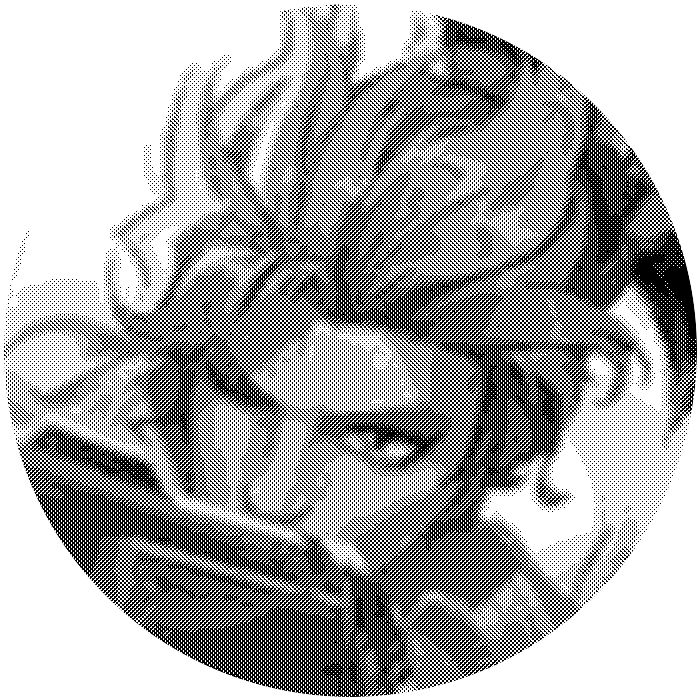
\includegraphics[width=1.35cm]{figures/icon-elsa-bloodstone.png}};
  \fill (1,0.72) -- (0.88,0.86) -- (1.12,0.86) -- cycle;
  \fill (6,0.72) -- (5.88,0.86) -- (6.12,0.86) -- cycle;
  \fill[black!22] (0,0.08) rectangle (2,0.62);
  \fill[black!58] (2,0.08) rectangle (10,0.62);
  \draw[|-|, thick] (0,0) -- (10,0);
  \node[anchor=north] at (1,-0.06) {Spider-Man, 2 min};
  \node[anchor=north] at (6,-0.06) {Elsa Bloodstone, 8 min};
  \node[anchor=east] at (-0.15,0.35) {Start};
  \node[anchor=west] at (10.15,0.35) {End};
  \tikzset{rule/.style={draw, align=center, text width=3.4cm, inner sep=4pt, minimum height=2.15cm, anchor=north}}
  \node[rule, thick] at (1.55,-0.85)
    {\textbf{Starting hero}\\{\footnotesize used in this report (W0)}\\[3pt] 100\% Spider-Man\\[3pt] {\footnotesize\itshape ``What did the team open with?''}};
  \node[rule] at (5,-0.85)
    {\textbf{Most-played hero}\\{\footnotesize (W2)}\\[3pt] 100\% Elsa Bloodstone\\[3pt] {\footnotesize\itshape ``What was played longest?''}};
  \node[rule] at (8.45,-0.85)
    {\textbf{Time-weighted}\\{\footnotesize (W1)}\\[3pt] 20\% Spider-Man, 80\% Elsa\\[3pt] {\footnotesize\itshape ``How were the minutes split?''}};
\end{tikzpicture}
\caption{Three ways to credit one player who swaps heroes. Illustrative; no estimation is involved.
The starting-hero rule is the one used here. Every lineup-derived quantity in the model (hero contrasts,
composition, allied pairs, opposing pairs) uses the same starting record.}
\label{fig:swap}
\end{figure}

The distinction matters because switching can respond to how the match develops. A player who is
losing a matchup, or who sees the opposing team change composition, may swap; the minutes they end up on
each hero are then partly a consequence of the match rather than a description of its starting
conditions. The opening and the eventual allocation of minutes therefore answer different questions. This
report asks the first one. The starting record carries its own limitation: a player who abandons a hero
after thirty seconds still counts as having started it, so the estimates describe the consequences of
opening with a hero, swaps included, rather than the hero's performance in uninterrupted play.

\subsection*{What the model adjusts for}

The model predicts the probability that side~0 wins a match from the two starting lineups and pre-match
information. Beyond each hero's own contrast it includes the map, the difference in the two teams' mean
pre-match rank score, the lobby's overall rank, the role composition of each team (how many Tanks, Damage
heroes, and Supports), every pair of allied starters, every pair of opposing starters, and a deviation for
each hero on each map. Hero, composition, and pair effects are all allowed to change linearly with lobby
rank. With <<N_FREE>> coefficients on <<N_DEV>> matches, the pair and rank-slope blocks are shrunk toward
zero by ridge penalties whose strengths were chosen on chronological development folds. Designated
team-ups are labels attached afterward; they receive no special treatment in estimation.

\section*{Which heroes have the largest estimated replacement values?}

Figure~\ref{fig:repl} shows the central quantity of the report. For each hero,
the model takes actual starting slots occupied by a hero of the same role, puts the hero into that slot
instead, keeps the slot's player, rank, map, side, and the other eleven starters fixed, recomputes every
affected term, and averages the change in predicted win probability. The benchmark is the average legal
same-role hero for that slot, so a value of <<MANTIS_CR>> for Mantis means that, averaged over the slots
where Mantis could legally have started, starting Mantis instead of an average available Support raises
the predicted win probability by <<MANTIS_CR>> percentage points. A positive value is an average model
prediction over those contexts, not a bonus that every lineup would receive.

\begin{figure}[H]\centering
\caption{Replacement values against the average legal same-role hero, all 55 heroes}\label{fig:repl}
\vspace{2pt}
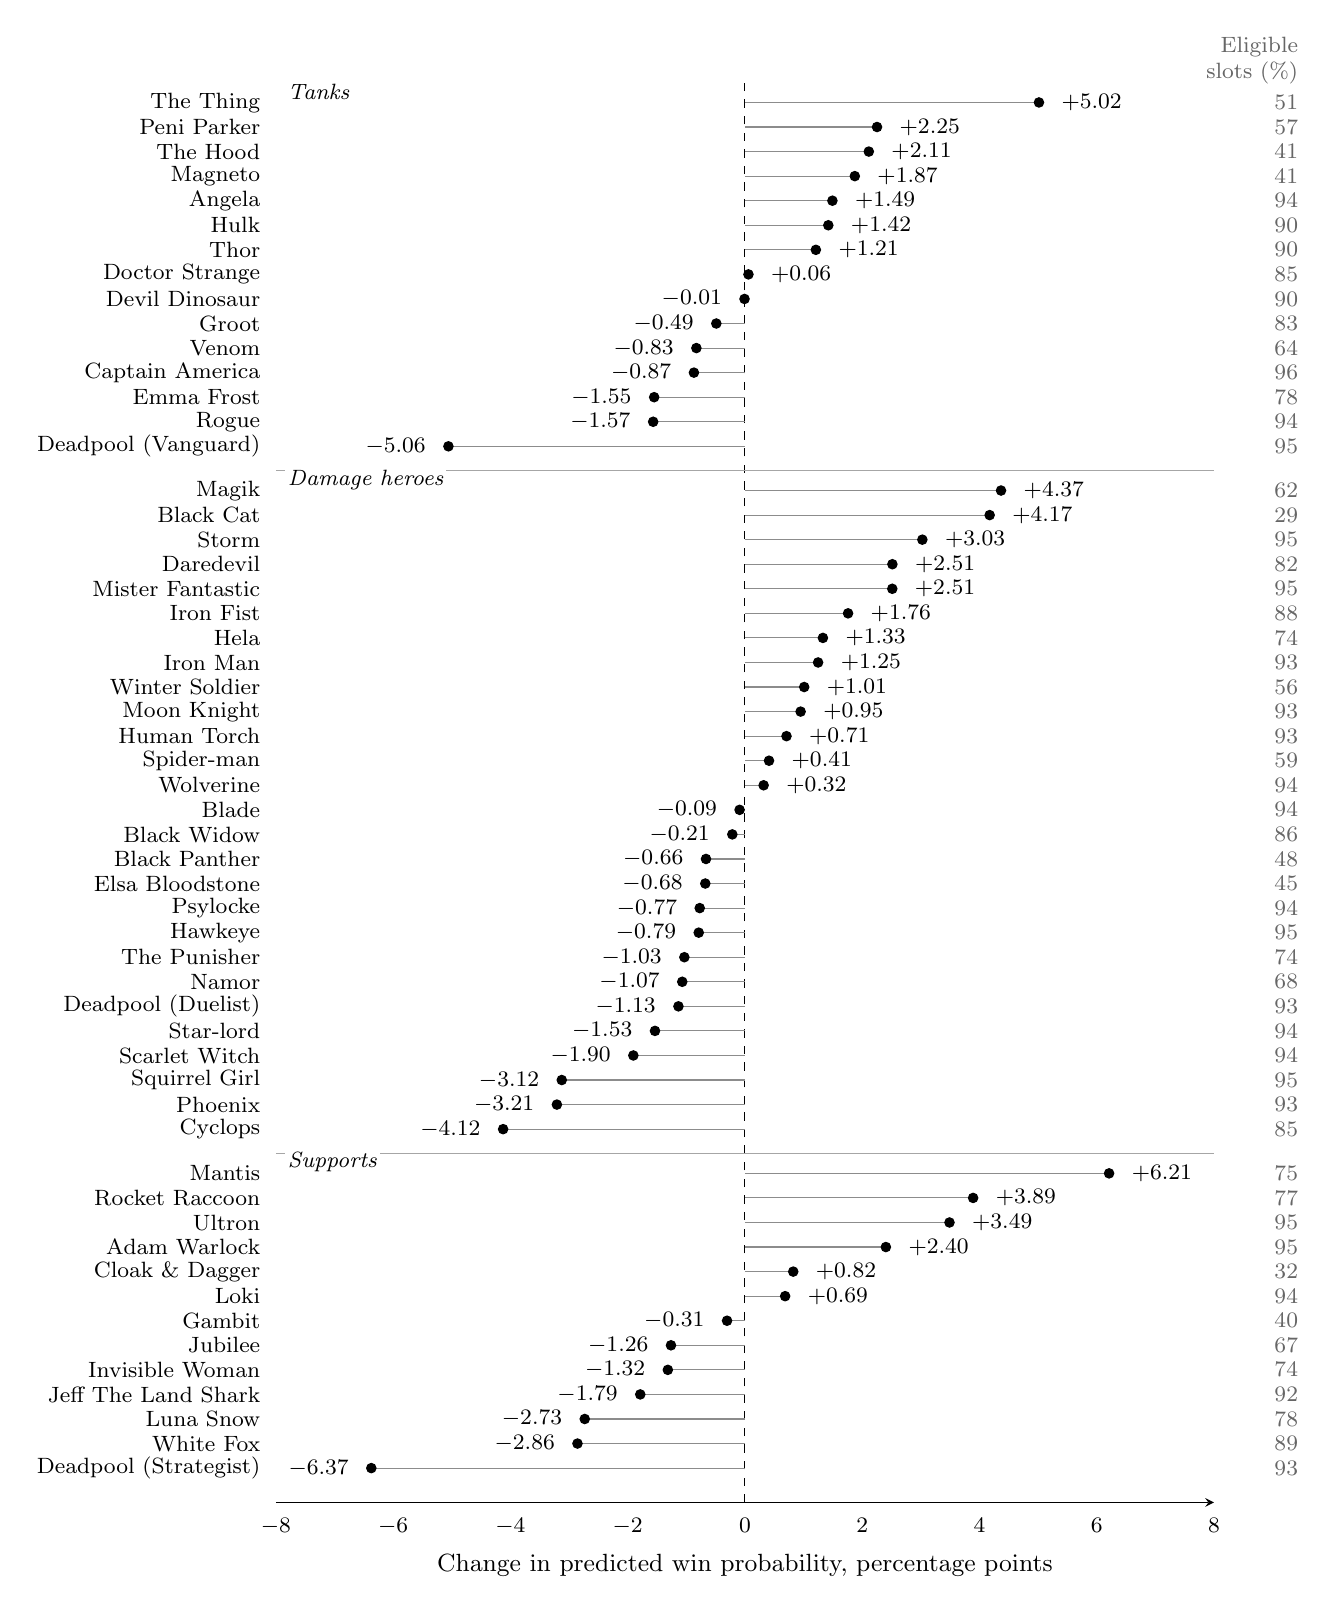
\begin{tikzpicture}
\begin{axis}[
  width=339.0pt, height=513.0pt, scale only axis, axis lines=left, tick style={draw=none}, y axis line style={draw=none}, clip=false,
  label style={font=\small}, tick label style={font=\footnotesize}, yticklabel style={font=\footnotesize},
  legend style={draw=none, fill=none, font=\footnotesize, cells={anchor=west}}, legend cell align=left,
  xmin=-8, xmax=8, ymin=0, ymax=57.80, xtick={-8,-6,...,8},
  xlabel={Change in predicted win probability, percentage points},
  ytick={57.00,56.00,55.00,54.00,53.00,52.00,51.00,50.00,49.00,48.00,47.00,46.00,45.00,44.00,43.00,41.20,40.20,39.20,38.20,37.20,36.20,35.20,34.20,33.20,32.20,31.20,30.20,29.20,28.20,27.20,26.20,25.20,24.20,23.20,22.20,21.20,20.20,19.20,18.20,17.20,16.20,15.20,13.40,12.40,11.40,10.40,9.40,8.40,7.40,6.40,5.40,4.40,3.40,2.40,1.40}, yticklabels={{The Thing},{Peni Parker},{The Hood},{Magneto},{Angela},{Hulk},{Thor},{Doctor Strange},{Devil Dinosaur},{Groot},{Venom},{Captain America},{Emma Frost},{Rogue},{Deadpool (Vanguard)},{Magik},{Black Cat},{Storm},{Daredevil},{Mister Fantastic},{Iron Fist},{Hela},{Iron Man},{Winter Soldier},{Moon Knight},{Human Torch},{Spider-man},{Wolverine},{Blade},{Black Widow},{Black Panther},{Elsa Bloodstone},{Psylocke},{Hawkeye},{The Punisher},{Namor},{Deadpool (Duelist)},{Star-lord},{Scarlet Witch},{Squirrel Girl},{Phoenix},{Cyclops},{Mantis},{Rocket Raccoon},{Ultron},{Adam Warlock},{Cloak \& Dagger},{Loki},{Gambit},{Jubilee},{Invisible Woman},{Jeff The Land Shark},{Luna Snow},{White Fox},{Deadpool (Strategist)}},
]
\draw[dashed, thin] (axis cs:0,0) -- (axis cs:0,57.80);
\draw[black!35, thin] (axis cs:-8,42.00) -- (axis cs:8,42.00);
\draw[black!35, thin] (axis cs:-8,14.20) -- (axis cs:8,14.20);
\draw[black!45, thin] (axis cs:0,57.00) -- (axis cs:5.015,57.00);
\draw[black!45, thin] (axis cs:0,56.00) -- (axis cs:2.253,56.00);
\draw[black!45, thin] (axis cs:0,55.00) -- (axis cs:2.113,55.00);
\draw[black!45, thin] (axis cs:0,54.00) -- (axis cs:1.874,54.00);
\draw[black!45, thin] (axis cs:0,53.00) -- (axis cs:1.492,53.00);
\draw[black!45, thin] (axis cs:0,52.00) -- (axis cs:1.422,52.00);
\draw[black!45, thin] (axis cs:0,51.00) -- (axis cs:1.210,51.00);
\draw[black!45, thin] (axis cs:0,50.00) -- (axis cs:0.060,50.00);
\draw[black!45, thin] (axis cs:0,49.00) -- (axis cs:-0.007,49.00);
\draw[black!45, thin] (axis cs:0,48.00) -- (axis cs:-0.488,48.00);
\draw[black!45, thin] (axis cs:0,47.00) -- (axis cs:-0.828,47.00);
\draw[black!45, thin] (axis cs:0,46.00) -- (axis cs:-0.870,46.00);
\draw[black!45, thin] (axis cs:0,45.00) -- (axis cs:-1.548,45.00);
\draw[black!45, thin] (axis cs:0,44.00) -- (axis cs:-1.565,44.00);
\draw[black!45, thin] (axis cs:0,43.00) -- (axis cs:-5.057,43.00);
\draw[black!45, thin] (axis cs:0,41.20) -- (axis cs:4.368,41.20);
\draw[black!45, thin] (axis cs:0,40.20) -- (axis cs:4.174,40.20);
\draw[black!45, thin] (axis cs:0,39.20) -- (axis cs:3.026,39.20);
\draw[black!45, thin] (axis cs:0,38.20) -- (axis cs:2.515,38.20);
\draw[black!45, thin] (axis cs:0,37.20) -- (axis cs:2.513,37.20);
\draw[black!45, thin] (axis cs:0,36.20) -- (axis cs:1.759,36.20);
\draw[black!45, thin] (axis cs:0,35.20) -- (axis cs:1.330,35.20);
\draw[black!45, thin] (axis cs:0,34.20) -- (axis cs:1.248,34.20);
\draw[black!45, thin] (axis cs:0,33.20) -- (axis cs:1.011,33.20);
\draw[black!45, thin] (axis cs:0,32.20) -- (axis cs:0.950,32.20);
\draw[black!45, thin] (axis cs:0,31.20) -- (axis cs:0.709,31.20);
\draw[black!45, thin] (axis cs:0,30.20) -- (axis cs:0.411,30.20);
\draw[black!45, thin] (axis cs:0,29.20) -- (axis cs:0.319,29.20);
\draw[black!45, thin] (axis cs:0,28.20) -- (axis cs:-0.091,28.20);
\draw[black!45, thin] (axis cs:0,27.20) -- (axis cs:-0.215,27.20);
\draw[black!45, thin] (axis cs:0,26.20) -- (axis cs:-0.664,26.20);
\draw[black!45, thin] (axis cs:0,25.20) -- (axis cs:-0.676,25.20);
\draw[black!45, thin] (axis cs:0,24.20) -- (axis cs:-0.771,24.20);
\draw[black!45, thin] (axis cs:0,23.20) -- (axis cs:-0.788,23.20);
\draw[black!45, thin] (axis cs:0,22.20) -- (axis cs:-1.033,22.20);
\draw[black!45, thin] (axis cs:0,21.20) -- (axis cs:-1.069,21.20);
\draw[black!45, thin] (axis cs:0,20.20) -- (axis cs:-1.134,20.20);
\draw[black!45, thin] (axis cs:0,19.20) -- (axis cs:-1.534,19.20);
\draw[black!45, thin] (axis cs:0,18.20) -- (axis cs:-1.903,18.20);
\draw[black!45, thin] (axis cs:0,17.20) -- (axis cs:-3.124,17.20);
\draw[black!45, thin] (axis cs:0,16.20) -- (axis cs:-3.207,16.20);
\draw[black!45, thin] (axis cs:0,15.20) -- (axis cs:-4.124,15.20);
\draw[black!45, thin] (axis cs:0,13.40) -- (axis cs:6.211,13.40);
\draw[black!45, thin] (axis cs:0,12.40) -- (axis cs:3.892,12.40);
\draw[black!45, thin] (axis cs:0,11.40) -- (axis cs:3.489,11.40);
\draw[black!45, thin] (axis cs:0,10.40) -- (axis cs:2.404,10.40);
\draw[black!45, thin] (axis cs:0,9.40) -- (axis cs:0.824,9.40);
\draw[black!45, thin] (axis cs:0,8.40) -- (axis cs:0.686,8.40);
\draw[black!45, thin] (axis cs:0,7.40) -- (axis cs:-0.305,7.40);
\draw[black!45, thin] (axis cs:0,6.40) -- (axis cs:-1.261,6.40);
\draw[black!45, thin] (axis cs:0,5.40) -- (axis cs:-1.315,5.40);
\draw[black!45, thin] (axis cs:0,4.40) -- (axis cs:-1.785,4.40);
\draw[black!45, thin] (axis cs:0,3.40) -- (axis cs:-2.732,3.40);
\draw[black!45, thin] (axis cs:0,2.40) -- (axis cs:-2.856,2.40);
\draw[black!45, thin] (axis cs:0,1.40) -- (axis cs:-6.372,1.40);
\addplot[only marks, mark=*, mark size=1.7pt] coordinates {
(5.015,57.00)
(2.253,56.00)
(2.113,55.00)
(1.874,54.00)
(1.492,53.00)
(1.422,52.00)
(1.210,51.00)
(0.060,50.00)
(-0.007,49.00)
(-0.488,48.00)
(-0.828,47.00)
(-0.870,46.00)
(-1.548,45.00)
(-1.565,44.00)
(-5.057,43.00)
(4.368,41.20)
(4.174,40.20)
(3.026,39.20)
(2.515,38.20)
(2.513,37.20)
(1.759,36.20)
(1.330,35.20)
(1.248,34.20)
(1.011,33.20)
(0.950,32.20)
(0.709,31.20)
(0.411,30.20)
(0.319,29.20)
(-0.091,28.20)
(-0.215,27.20)
(-0.664,26.20)
(-0.676,25.20)
(-0.771,24.20)
(-0.788,23.20)
(-1.033,22.20)
(-1.069,21.20)
(-1.134,20.20)
(-1.534,19.20)
(-1.903,18.20)
(-3.124,17.20)
(-3.207,16.20)
(-4.124,15.20)
(6.211,13.40)
(3.892,12.40)
(3.489,11.40)
(2.404,10.40)
(0.824,9.40)
(0.686,8.40)
(-0.305,7.40)
(-1.261,6.40)
(-1.315,5.40)
(-1.785,4.40)
(-2.732,3.40)
(-2.856,2.40)
(-6.372,1.40)
};
\node[anchor=west, font=\footnotesize\itshape, fill=white, inner sep=1pt] at (axis cs:-7.85,57.45) {Tanks};
\node[anchor=west, font=\footnotesize\itshape, fill=white, inner sep=1pt] at (axis cs:-7.85,41.65) {Damage heroes};
\node[anchor=west, font=\footnotesize\itshape, fill=white, inner sep=1pt] at (axis cs:-7.85,13.85) {Supports};
\node[anchor=west, font=\footnotesize] at (axis cs:5.235,57.00) {+5.02};
\node[anchor=west, font=\footnotesize] at (axis cs:2.473,56.00) {+2.25};
\node[anchor=west, font=\footnotesize] at (axis cs:2.333,55.00) {+2.11};
\node[anchor=west, font=\footnotesize] at (axis cs:2.094,54.00) {+1.87};
\node[anchor=west, font=\footnotesize] at (axis cs:1.712,53.00) {+1.49};
\node[anchor=west, font=\footnotesize] at (axis cs:1.642,52.00) {+1.42};
\node[anchor=west, font=\footnotesize] at (axis cs:1.430,51.00) {+1.21};
\node[anchor=west, font=\footnotesize] at (axis cs:0.280,50.00) {+0.06};
\node[anchor=east, font=\footnotesize] at (axis cs:-0.227,49.00) {$-$0.01};
\node[anchor=east, font=\footnotesize] at (axis cs:-0.708,48.00) {$-$0.49};
\node[anchor=east, font=\footnotesize] at (axis cs:-1.048,47.00) {$-$0.83};
\node[anchor=east, font=\footnotesize] at (axis cs:-1.090,46.00) {$-$0.87};
\node[anchor=east, font=\footnotesize] at (axis cs:-1.768,45.00) {$-$1.55};
\node[anchor=east, font=\footnotesize] at (axis cs:-1.785,44.00) {$-$1.57};
\node[anchor=east, font=\footnotesize] at (axis cs:-5.277,43.00) {$-$5.06};
\node[anchor=west, font=\footnotesize] at (axis cs:4.588,41.20) {+4.37};
\node[anchor=west, font=\footnotesize] at (axis cs:4.394,40.20) {+4.17};
\node[anchor=west, font=\footnotesize] at (axis cs:3.246,39.20) {+3.03};
\node[anchor=west, font=\footnotesize] at (axis cs:2.735,38.20) {+2.51};
\node[anchor=west, font=\footnotesize] at (axis cs:2.733,37.20) {+2.51};
\node[anchor=west, font=\footnotesize] at (axis cs:1.979,36.20) {+1.76};
\node[anchor=west, font=\footnotesize] at (axis cs:1.550,35.20) {+1.33};
\node[anchor=west, font=\footnotesize] at (axis cs:1.468,34.20) {+1.25};
\node[anchor=west, font=\footnotesize] at (axis cs:1.231,33.20) {+1.01};
\node[anchor=west, font=\footnotesize] at (axis cs:1.170,32.20) {+0.95};
\node[anchor=west, font=\footnotesize] at (axis cs:0.929,31.20) {+0.71};
\node[anchor=west, font=\footnotesize] at (axis cs:0.631,30.20) {+0.41};
\node[anchor=west, font=\footnotesize] at (axis cs:0.539,29.20) {+0.32};
\node[anchor=east, font=\footnotesize] at (axis cs:-0.311,28.20) {$-$0.09};
\node[anchor=east, font=\footnotesize] at (axis cs:-0.435,27.20) {$-$0.21};
\node[anchor=east, font=\footnotesize] at (axis cs:-0.884,26.20) {$-$0.66};
\node[anchor=east, font=\footnotesize] at (axis cs:-0.896,25.20) {$-$0.68};
\node[anchor=east, font=\footnotesize] at (axis cs:-0.991,24.20) {$-$0.77};
\node[anchor=east, font=\footnotesize] at (axis cs:-1.008,23.20) {$-$0.79};
\node[anchor=east, font=\footnotesize] at (axis cs:-1.253,22.20) {$-$1.03};
\node[anchor=east, font=\footnotesize] at (axis cs:-1.289,21.20) {$-$1.07};
\node[anchor=east, font=\footnotesize] at (axis cs:-1.354,20.20) {$-$1.13};
\node[anchor=east, font=\footnotesize] at (axis cs:-1.754,19.20) {$-$1.53};
\node[anchor=east, font=\footnotesize] at (axis cs:-2.123,18.20) {$-$1.90};
\node[anchor=east, font=\footnotesize] at (axis cs:-3.344,17.20) {$-$3.12};
\node[anchor=east, font=\footnotesize] at (axis cs:-3.427,16.20) {$-$3.21};
\node[anchor=east, font=\footnotesize] at (axis cs:-4.344,15.20) {$-$4.12};
\node[anchor=west, font=\footnotesize] at (axis cs:6.431,13.40) {+6.21};
\node[anchor=west, font=\footnotesize] at (axis cs:4.112,12.40) {+3.89};
\node[anchor=west, font=\footnotesize] at (axis cs:3.709,11.40) {+3.49};
\node[anchor=west, font=\footnotesize] at (axis cs:2.624,10.40) {+2.40};
\node[anchor=west, font=\footnotesize] at (axis cs:1.044,9.40) {+0.82};
\node[anchor=west, font=\footnotesize] at (axis cs:0.906,8.40) {+0.69};
\node[anchor=east, font=\footnotesize] at (axis cs:-0.525,7.40) {$-$0.31};
\node[anchor=east, font=\footnotesize] at (axis cs:-1.481,6.40) {$-$1.26};
\node[anchor=east, font=\footnotesize] at (axis cs:-1.535,5.40) {$-$1.32};
\node[anchor=east, font=\footnotesize] at (axis cs:-2.005,4.40) {$-$1.79};
\node[anchor=east, font=\footnotesize] at (axis cs:-2.952,3.40) {$-$2.73};
\node[anchor=east, font=\footnotesize] at (axis cs:-3.076,2.40) {$-$2.86};
\node[anchor=east, font=\footnotesize] at (axis cs:-6.592,1.40) {$-$6.37};
\node[anchor=south east, font=\footnotesize, text=black!60, align=right] at (axis cs:9.6,57.35) {Eligible\\ slots (\%)};
\node[anchor=east, font=\footnotesize, text=black!60] at (axis cs:9.6,57.00) {51};
\node[anchor=east, font=\footnotesize, text=black!60] at (axis cs:9.6,56.00) {57};
\node[anchor=east, font=\footnotesize, text=black!60] at (axis cs:9.6,55.00) {41};
\node[anchor=east, font=\footnotesize, text=black!60] at (axis cs:9.6,54.00) {41};
\node[anchor=east, font=\footnotesize, text=black!60] at (axis cs:9.6,53.00) {94};
\node[anchor=east, font=\footnotesize, text=black!60] at (axis cs:9.6,52.00) {90};
\node[anchor=east, font=\footnotesize, text=black!60] at (axis cs:9.6,51.00) {90};
\node[anchor=east, font=\footnotesize, text=black!60] at (axis cs:9.6,50.00) {85};
\node[anchor=east, font=\footnotesize, text=black!60] at (axis cs:9.6,49.00) {90};
\node[anchor=east, font=\footnotesize, text=black!60] at (axis cs:9.6,48.00) {83};
\node[anchor=east, font=\footnotesize, text=black!60] at (axis cs:9.6,47.00) {64};
\node[anchor=east, font=\footnotesize, text=black!60] at (axis cs:9.6,46.00) {96};
\node[anchor=east, font=\footnotesize, text=black!60] at (axis cs:9.6,45.00) {78};
\node[anchor=east, font=\footnotesize, text=black!60] at (axis cs:9.6,44.00) {94};
\node[anchor=east, font=\footnotesize, text=black!60] at (axis cs:9.6,43.00) {95};
\node[anchor=east, font=\footnotesize, text=black!60] at (axis cs:9.6,41.20) {62};
\node[anchor=east, font=\footnotesize, text=black!60] at (axis cs:9.6,40.20) {29};
\node[anchor=east, font=\footnotesize, text=black!60] at (axis cs:9.6,39.20) {95};
\node[anchor=east, font=\footnotesize, text=black!60] at (axis cs:9.6,38.20) {82};
\node[anchor=east, font=\footnotesize, text=black!60] at (axis cs:9.6,37.20) {95};
\node[anchor=east, font=\footnotesize, text=black!60] at (axis cs:9.6,36.20) {88};
\node[anchor=east, font=\footnotesize, text=black!60] at (axis cs:9.6,35.20) {74};
\node[anchor=east, font=\footnotesize, text=black!60] at (axis cs:9.6,34.20) {93};
\node[anchor=east, font=\footnotesize, text=black!60] at (axis cs:9.6,33.20) {56};
\node[anchor=east, font=\footnotesize, text=black!60] at (axis cs:9.6,32.20) {93};
\node[anchor=east, font=\footnotesize, text=black!60] at (axis cs:9.6,31.20) {93};
\node[anchor=east, font=\footnotesize, text=black!60] at (axis cs:9.6,30.20) {59};
\node[anchor=east, font=\footnotesize, text=black!60] at (axis cs:9.6,29.20) {94};
\node[anchor=east, font=\footnotesize, text=black!60] at (axis cs:9.6,28.20) {94};
\node[anchor=east, font=\footnotesize, text=black!60] at (axis cs:9.6,27.20) {86};
\node[anchor=east, font=\footnotesize, text=black!60] at (axis cs:9.6,26.20) {48};
\node[anchor=east, font=\footnotesize, text=black!60] at (axis cs:9.6,25.20) {45};
\node[anchor=east, font=\footnotesize, text=black!60] at (axis cs:9.6,24.20) {94};
\node[anchor=east, font=\footnotesize, text=black!60] at (axis cs:9.6,23.20) {95};
\node[anchor=east, font=\footnotesize, text=black!60] at (axis cs:9.6,22.20) {74};
\node[anchor=east, font=\footnotesize, text=black!60] at (axis cs:9.6,21.20) {68};
\node[anchor=east, font=\footnotesize, text=black!60] at (axis cs:9.6,20.20) {93};
\node[anchor=east, font=\footnotesize, text=black!60] at (axis cs:9.6,19.20) {94};
\node[anchor=east, font=\footnotesize, text=black!60] at (axis cs:9.6,18.20) {94};
\node[anchor=east, font=\footnotesize, text=black!60] at (axis cs:9.6,17.20) {95};
\node[anchor=east, font=\footnotesize, text=black!60] at (axis cs:9.6,16.20) {93};
\node[anchor=east, font=\footnotesize, text=black!60] at (axis cs:9.6,15.20) {85};
\node[anchor=east, font=\footnotesize, text=black!60] at (axis cs:9.6,13.40) {75};
\node[anchor=east, font=\footnotesize, text=black!60] at (axis cs:9.6,12.40) {77};
\node[anchor=east, font=\footnotesize, text=black!60] at (axis cs:9.6,11.40) {95};
\node[anchor=east, font=\footnotesize, text=black!60] at (axis cs:9.6,10.40) {95};
\node[anchor=east, font=\footnotesize, text=black!60] at (axis cs:9.6,9.40) {32};
\node[anchor=east, font=\footnotesize, text=black!60] at (axis cs:9.6,8.40) {94};
\node[anchor=east, font=\footnotesize, text=black!60] at (axis cs:9.6,7.40) {40};
\node[anchor=east, font=\footnotesize, text=black!60] at (axis cs:9.6,6.40) {67};
\node[anchor=east, font=\footnotesize, text=black!60] at (axis cs:9.6,5.40) {74};
\node[anchor=east, font=\footnotesize, text=black!60] at (axis cs:9.6,4.40) {92};
\node[anchor=east, font=\footnotesize, text=black!60] at (axis cs:9.6,3.40) {78};
\node[anchor=east, font=\footnotesize, text=black!60] at (axis cs:9.6,2.40) {89};
\node[anchor=east, font=\footnotesize, text=black!60] at (axis cs:9.6,1.40) {93};
\end{axis}
\end{tikzpicture}


\begin{minipage}{0.95\linewidth}\footnotesize\vspace{2pt}
\emph{Notes.} Each dot is the average change in predicted win probability, in percentage points, when the
hero replaces the average legal same-role hero in the same starting slot, over <<POOL_N>> development
matches; heroes are sorted within role. \emph{Eligible slots} is the share of same-role slots in which the
hero was a legal replacement (not already on that side and not banned in that match); each hero's average
runs over its own eligible subset. No uncertainty has been computed for these values, so close neighbours
should not be read as distinguishable.
\end{minipage}
\end{figure}

Within each role the spread is wide. Among Tanks the largest estimates are <<TOP_TANK>>, and the smallest
<<BOT_TANK>>. Among Damage heroes the largest are <<TOP_DMG>> and the smallest <<BOT_DMG>>. Among
Supports, Mantis leads at <<MANTIS_CR>>, followed by <<TOP_SUP2>>, with <<BOT_SUP>> at the bottom. These are
the largest fitted values within their roles; without effect uncertainty the report does not claim that
heroes a few tenths of a point apart differ.

Two benchmarks are available, and they can disagree for the same hero. Doctor Strange is the clearest
case, shown in Table~\ref{tab:strange}: approximately neutral against the legal same-role reference at
<<STRANGE_CR>> percentage points, but <<STRANGE_OM>> points against the heroes actually selected in the
evaluated slots. Both numbers come from the same model. They differ because the alternative being replaced
differs: Tank slots in the sample are disproportionately filled by strong Tanks, so replacing the actual
incumbent is a harder comparison than replacing an average of everything legal.

\begin{table}[H]\centering\small
\caption{Two replacement benchmarks for Doctor Strange, from the same fit}\label{tab:strange}
\begin{tabular}{l l r}
\toprule
Benchmark & Alternative being replaced & Value, pp \\
\midrule
Common reference & the average legal same-role hero in the slot & <<STRANGE_CR>> \\
Observed incumbent & the Tank who actually started in the slot & <<STRANGE_OM>> \\
\bottomrule
\end{tabular}
\end{table}

The averaging rule deserves a precise statement, because the two benchmarks share a context pool but not a
context set. The pool is <<POOL_N>> development matches. For a given hero, the contexts are every starting
slot in those matches occupied by a same-role hero, and a context is eligible only if the hero was not
already on that side and was not banned in that match. Each hero's value is the mean over its own eligible
contexts, so heroes differ in which slots they are scored on. Bans drive most of the difference: Black Cat
is eligible in <<BLACKCAT_COV>> of Damage slots, against <<WOLV_COV>> for Wolverine, because she is banned
so often. The common reference compares the hero with the average of the same-role heroes that were legal
in that slot, computed slot by slot, which is why it is the fairer of the two for ranking heroes, while the
observed-incumbent benchmark answers the more literal question of what would have happened in the slots as
they were actually filled.

\section*{How do those values differ across rank environments?}

The replacement values can also be averaged within thirds of the sample by lobby rank, the mean pre-match
score of the twelve starters, with cutoffs at <<THIRD_LO>> and <<THIRD_HI>>. Figure~\ref{fig:rank} shows
the heroes whose observed-incumbent value changes most between the lower and upper thirds: the four
largest increases and the four largest decreases, which is the selection rule and the only one. The
full roster is in Appendix Figure~\ref{fig:rank-all}.

\begin{figure}[H]\centering
\caption{Heroes whose replacement value changes most between the lower and upper thirds by lobby rank}
\label{fig:rank}
\vspace{2pt}
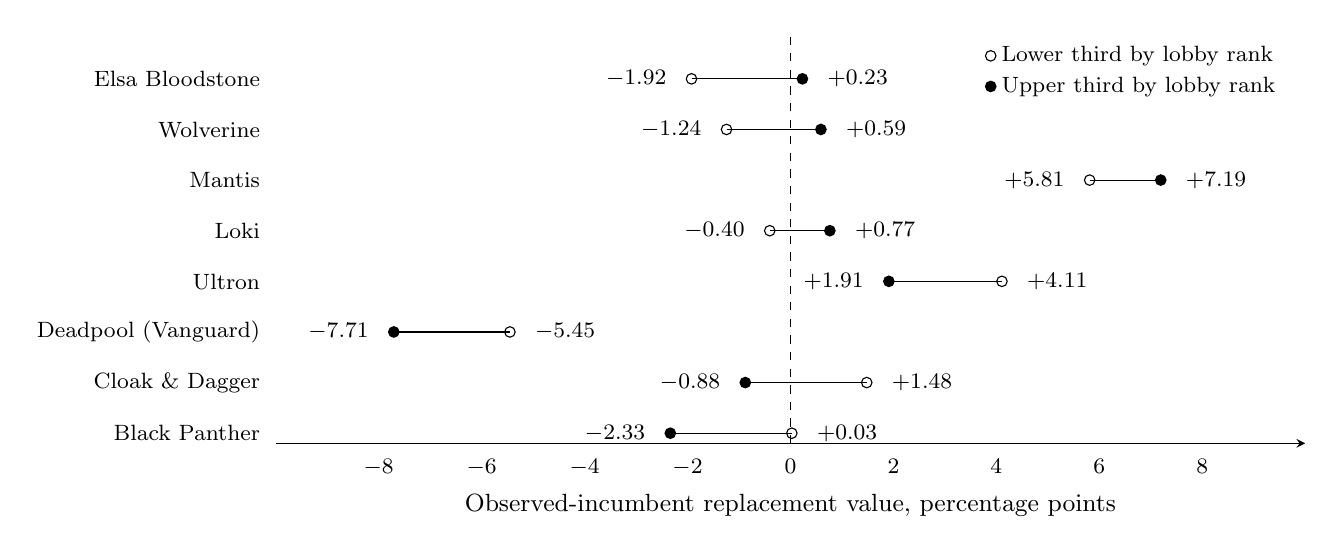
\begin{tikzpicture}
\begin{axis}[
  width=372.0pt, height=150.0pt, scale only axis, axis lines=left, tick style={draw=none}, y axis line style={draw=none}, clip=false,
  label style={font=\small}, tick label style={font=\footnotesize}, yticklabel style={font=\footnotesize},
  legend style={draw=none, fill=none, font=\footnotesize, cells={anchor=west}}, legend cell align=left,
  xmin=-10, xmax=10, ymin=0.4, ymax=8.60, xtick={-8,-6,...,8},
  xlabel={Observed-incumbent replacement value, percentage points},
  ytick={7.60,6.60,5.60,4.60,3.60,2.60,1.60,0.60}, yticklabels={{Elsa Bloodstone},{Wolverine},{Mantis},{Loki},{Ultron},{Deadpool (Vanguard)},{Cloak \& Dagger},{Black Panther}},
  legend style={at={(0.985,0.985)}, anchor=north east},
]
\draw[dashed, thin] (axis cs:0,0.4) -- (axis cs:0,8.60);
\draw[thin] (axis cs:-1.922,7.60) -- (axis cs:0.233,7.60);
\draw[thin] (axis cs:-1.242,6.60) -- (axis cs:0.592,6.60);
\draw[thin] (axis cs:5.813,5.60) -- (axis cs:7.194,5.60);
\draw[thin] (axis cs:-0.402,4.60) -- (axis cs:0.766,4.60);
\draw[thin] (axis cs:4.109,3.60) -- (axis cs:1.912,3.60);
\draw[thin] (axis cs:-5.450,2.60) -- (axis cs:-7.706,2.60);
\draw[thin] (axis cs:1.482,1.60) -- (axis cs:-0.877,1.60);
\draw[thin] (axis cs:0.027,0.60) -- (axis cs:-2.334,0.60);
\addplot[only marks, mark=o, mark size=1.9pt] coordinates {
(-1.922,7.60)
(-1.242,6.60)
(5.813,5.60)
(-0.402,4.60)
(4.109,3.60)
(-5.450,2.60)
(1.482,1.60)
(0.027,0.60)
};
\addlegendentry{Lower third by lobby rank}
\addplot[only marks, mark=*, mark size=1.9pt] coordinates {
(0.233,7.60)
(0.592,6.60)
(7.194,5.60)
(0.766,4.60)
(1.912,3.60)
(-7.706,2.60)
(-0.877,1.60)
(-2.334,0.60)
};
\addlegendentry{Upper third by lobby rank}
\node[anchor=east, font=\footnotesize] at (axis cs:-2.222,7.60) {$-$1.92};
\node[anchor=west, font=\footnotesize] at (axis cs:0.533,7.60) {+0.23};
\node[anchor=east, font=\footnotesize] at (axis cs:-1.542,6.60) {$-$1.24};
\node[anchor=west, font=\footnotesize] at (axis cs:0.892,6.60) {+0.59};
\node[anchor=east, font=\footnotesize] at (axis cs:5.513,5.60) {+5.81};
\node[anchor=west, font=\footnotesize] at (axis cs:7.494,5.60) {+7.19};
\node[anchor=east, font=\footnotesize] at (axis cs:-0.702,4.60) {$-$0.40};
\node[anchor=west, font=\footnotesize] at (axis cs:1.066,4.60) {+0.77};
\node[anchor=east, font=\footnotesize] at (axis cs:1.612,3.60) {+1.91};
\node[anchor=west, font=\footnotesize] at (axis cs:4.409,3.60) {+4.11};
\node[anchor=east, font=\footnotesize] at (axis cs:-8.006,2.60) {$-$7.71};
\node[anchor=west, font=\footnotesize] at (axis cs:-5.150,2.60) {$-$5.45};
\node[anchor=east, font=\footnotesize] at (axis cs:-1.177,1.60) {$-$0.88};
\node[anchor=west, font=\footnotesize] at (axis cs:1.782,1.60) {+1.48};
\node[anchor=east, font=\footnotesize] at (axis cs:-2.634,0.60) {$-$2.33};
\node[anchor=west, font=\footnotesize] at (axis cs:0.327,0.60) {+0.03};
\end{axis}
\end{tikzpicture}


\begin{minipage}{0.95\linewidth}\footnotesize\vspace{2pt}
\emph{Notes.} Observed-incumbent replacement values averaged within the lower and upper thirds of sampled
lobbies by mean pre-match score (cut at <<THIRD_LO>> and <<THIRD_HI>>), for the four largest increases and
the four largest decreases among the 55 heroes. Each line joins two estimates from the same fit; it is not
a confidence interval, and no uncertainty has been computed for these values. Appendix
Figure~\ref{fig:rank-all} shows every hero.
\end{minipage}
\end{figure}

Elsa Bloodstone rises from <<ELSA_LO>> to <<ELSA_HI>> points, Wolverine from <<WOLV_LO>> to <<WOLV_HI>>,
and Mantis, already the strongest Support, from <<MANTIS_LO>> to <<MANTIS_HI>>. In the other direction,
Black Panther falls from <<BP_LO>> to <<BP_HI>>, Cloak \& Dagger from <<CD_LO>> to <<CD_HI>>, and Ultron
from <<ULTRON_LO>> to <<ULTRON_HI>>. In all, <<N_MOVE1>> of the 55 heroes move by at least one percentage
point between the two thirds.

These are variations across observed rank environments, and they should be read that way. The lobbies in
the upper third differ from those in the lower third in more than the players' skill: the compositions,
bans, maps, and opponents a hero meets all shift with rank, and the scores average over those contexts as
encountered. The figure does not isolate the mechanical effect of raising player skill while holding
everything else fixed. It also cannot speak to the top of the ladder, which is thinly sampled: the upper
third begins at a lobby mean of <<THIRD_HI>>, and few sampled lobbies average above 5{,}000.

\section*{Which teammates fit together, and which opposing matchups stand out?}

A pair effect is reported as a four-lineup contrast on the log-odds scale. Take the pair's coefficient,
subtract the average coefficient of each member with the same-role alternatives to the other, and add back
the average over alternative pairs. The result asks whether these two heroes add more together than their
separate relationships with other heroes would predict; it cancels the hero main effects and each hero's
other pairings, so it does not depend on where additive hero content is placed. These are log-odds
contrasts, not percentage-point contributions of the pair to a lineup: a four-lineup contrast compares
four hypothetical lineups, not one lineup with and without the pair. Figure~\ref{fig:pairs} shows selected
contrasts with the number of identifying matches, meaning distinct development matches in which the
pair's signed feature is nonzero; only pairs with at least <<MIN_SUPPORT>> such matches are shown.

\begin{figure}[H]\centering
\caption{Pair contrasts from the selected fit: designated team-ups, other allied pairs, opposing matchups}
\label{fig:pairs}
\vspace{2pt}
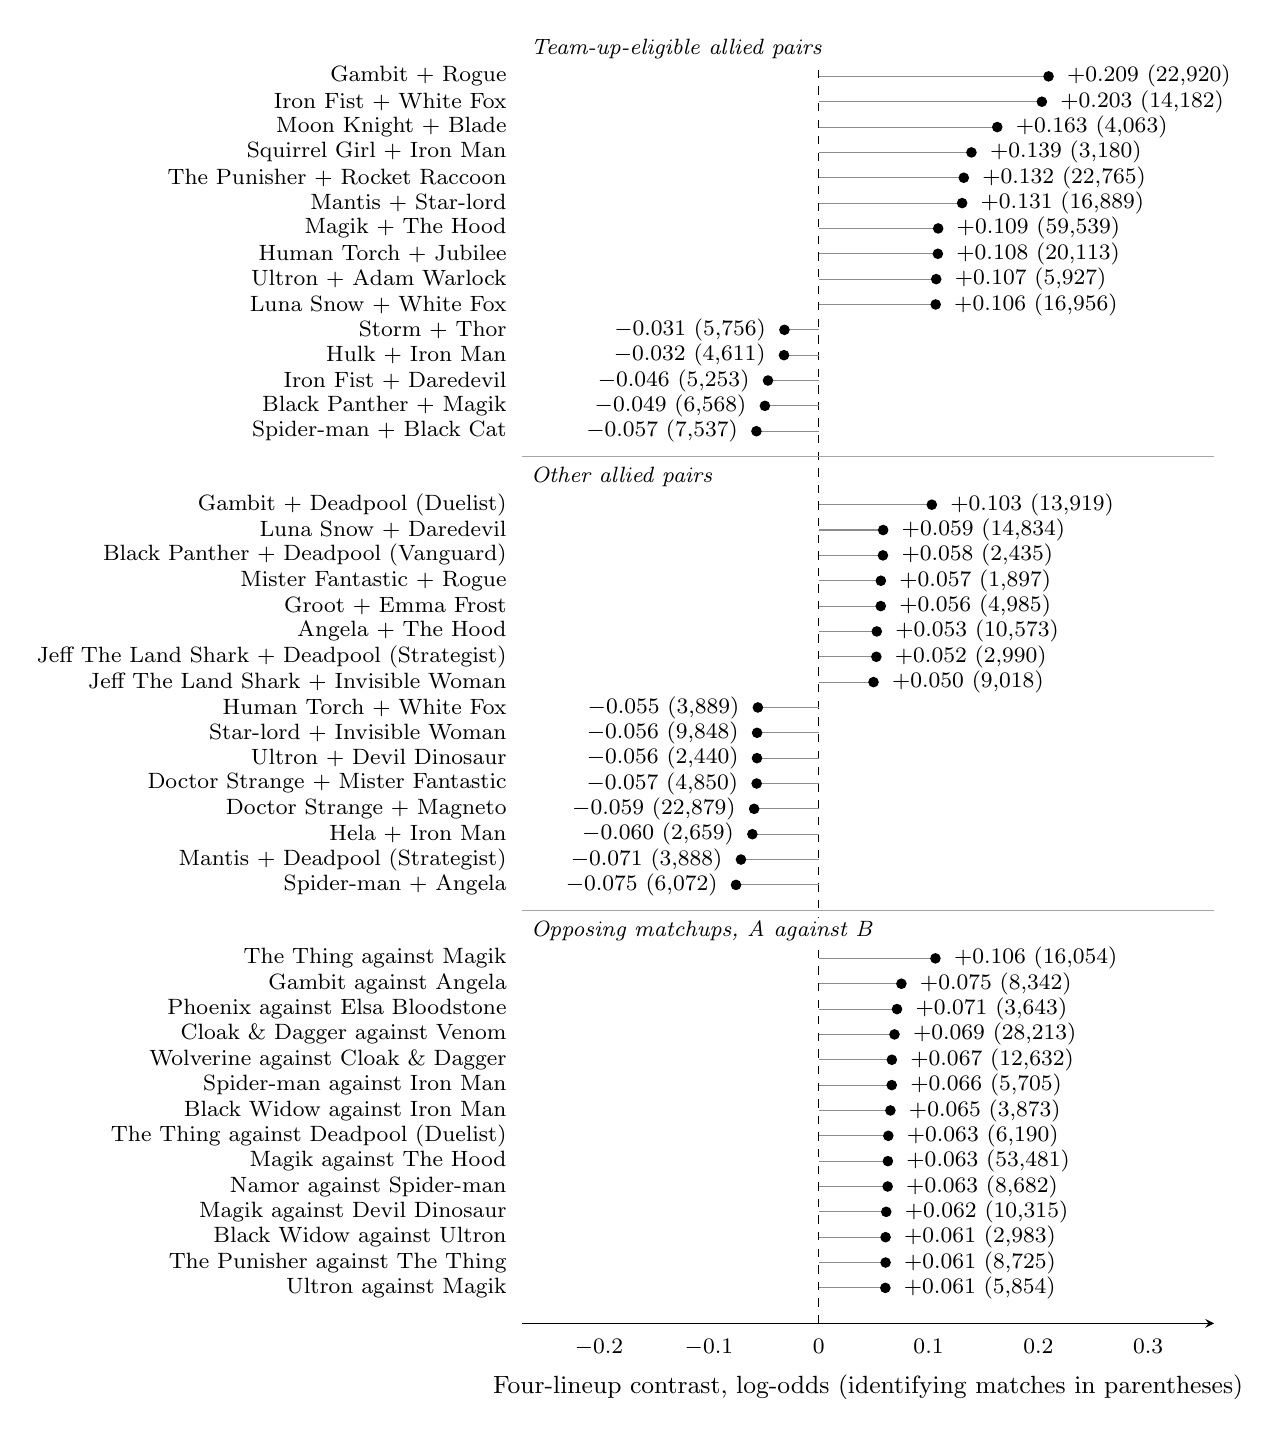
\begin{tikzpicture}
\begin{axis}[
  width=250.0pt, height=468.0pt, scale only axis, axis lines=left, tick style={draw=none}, y axis line style={draw=none}, clip=false,
  label style={font=\small}, tick label style={font=\footnotesize}, yticklabel style={font=\footnotesize},
  legend style={draw=none, fill=none, font=\footnotesize, cells={anchor=west}}, legend cell align=left,
  xmin=-0.27, xmax=0.36, ymin=0, ymax=51.10, xtick={-0.2,-0.1,...,0.3},
  xticklabel style={/pgf/number format/fixed, /pgf/number format/precision=1},
  xlabel={Four-lineup contrast, log-odds (identifying matches in parentheses)},
  ytick={49.20,48.20,47.20,46.20,45.20,44.20,43.20,42.20,41.20,40.20,39.20,38.20,37.20,36.20,35.20,32.30,31.30,30.30,29.30,28.30,27.30,26.30,25.30,24.30,23.30,22.30,21.30,20.30,19.30,18.30,17.30,14.40,13.40,12.40,11.40,10.40,9.40,8.40,7.40,6.40,5.40,4.40,3.40,2.40,1.40}, yticklabels={{Gambit + Rogue},{Iron Fist + White Fox},{Moon Knight + Blade},{Squirrel Girl + Iron Man},{The Punisher + Rocket Raccoon},{Mantis + Star-lord},{Magik + The Hood},{Human Torch + Jubilee},{Ultron + Adam Warlock},{Luna Snow + White Fox},{Storm + Thor},{Hulk + Iron Man},{Iron Fist + Daredevil},{Black Panther + Magik},{Spider-man + Black Cat},{Gambit + Deadpool (Duelist)},{Luna Snow + Daredevil},{Black Panther + Deadpool (Vanguard)},{Mister Fantastic + Rogue},{Groot + Emma Frost},{Angela + The Hood},{Jeff The Land Shark + Deadpool (Strategist)},{Jeff The Land Shark + Invisible Woman},{Human Torch + White Fox},{Star-lord + Invisible Woman},{Ultron + Devil Dinosaur},{Doctor Strange + Mister Fantastic},{Doctor Strange + Magneto},{Hela + Iron Man},{Mantis + Deadpool (Strategist)},{Spider-man + Angela},{The Thing against Magik},{Gambit against Angela},{Phoenix against Elsa Bloodstone},{Cloak \& Dagger against Venom},{Wolverine against Cloak \& Dagger},{Spider-man against Iron Man},{Black Widow against Iron Man},{The Thing against Deadpool (Duelist)},{Magik against The Hood},{Namor against Spider-man},{Magik against Devil Dinosaur},{Black Widow against Ultron},{The Punisher against The Thing},{Ultron against Magik}},
]
\draw[dashed, thin] (axis cs:0,0) -- (axis cs:0,51.10);
\draw[black!35, thin] (axis cs:-0.27,34.20) -- (axis cs:0.36,34.20);
\draw[black!35, thin] (axis cs:-0.27,16.30) -- (axis cs:0.36,16.30);
\draw[black!45, thin] (axis cs:0,49.20) -- (axis cs:0.2093,49.20);
\draw[black!45, thin] (axis cs:0,48.20) -- (axis cs:0.2032,48.20);
\draw[black!45, thin] (axis cs:0,47.20) -- (axis cs:0.1626,47.20);
\draw[black!45, thin] (axis cs:0,46.20) -- (axis cs:0.1391,46.20);
\draw[black!45, thin] (axis cs:0,45.20) -- (axis cs:0.1321,45.20);
\draw[black!45, thin] (axis cs:0,44.20) -- (axis cs:0.1306,44.20);
\draw[black!45, thin] (axis cs:0,43.20) -- (axis cs:0.1088,43.20);
\draw[black!45, thin] (axis cs:0,42.20) -- (axis cs:0.1085,42.20);
\draw[black!45, thin] (axis cs:0,41.20) -- (axis cs:0.1070,41.20);
\draw[black!45, thin] (axis cs:0,40.20) -- (axis cs:0.1065,40.20);
\draw[black!45, thin] (axis cs:0,39.20) -- (axis cs:-0.0312,39.20);
\draw[black!45, thin] (axis cs:0,38.20) -- (axis cs:-0.0316,38.20);
\draw[black!45, thin] (axis cs:0,37.20) -- (axis cs:-0.0462,37.20);
\draw[black!45, thin] (axis cs:0,36.20) -- (axis cs:-0.0490,36.20);
\draw[black!45, thin] (axis cs:0,35.20) -- (axis cs:-0.0567,35.20);
\draw[black!45, thin] (axis cs:0,32.30) -- (axis cs:0.1030,32.30);
\draw[black!45, thin] (axis cs:0,31.30) -- (axis cs:0.0587,31.30);
\draw[black!45, thin] (axis cs:0,30.30) -- (axis cs:0.0585,30.30);
\draw[black!45, thin] (axis cs:0,29.30) -- (axis cs:0.0566,29.30);
\draw[black!45, thin] (axis cs:0,28.30) -- (axis cs:0.0565,28.30);
\draw[black!45, thin] (axis cs:0,27.30) -- (axis cs:0.0529,27.30);
\draw[black!45, thin] (axis cs:0,26.30) -- (axis cs:0.0525,26.30);
\draw[black!45, thin] (axis cs:0,25.30) -- (axis cs:0.0499,25.30);
\draw[black!45, thin] (axis cs:0,24.30) -- (axis cs:-0.0554,24.30);
\draw[black!45, thin] (axis cs:0,23.30) -- (axis cs:-0.0561,23.30);
\draw[black!45, thin] (axis cs:0,22.30) -- (axis cs:-0.0562,22.30);
\draw[black!45, thin] (axis cs:0,21.30) -- (axis cs:-0.0565,21.30);
\draw[black!45, thin] (axis cs:0,20.30) -- (axis cs:-0.0588,20.30);
\draw[black!45, thin] (axis cs:0,19.30) -- (axis cs:-0.0604,19.30);
\draw[black!45, thin] (axis cs:0,18.30) -- (axis cs:-0.0708,18.30);
\draw[black!45, thin] (axis cs:0,17.30) -- (axis cs:-0.0753,17.30);
\draw[black!45, thin] (axis cs:0,14.40) -- (axis cs:0.1063,14.40);
\draw[black!45, thin] (axis cs:0,13.40) -- (axis cs:0.0753,13.40);
\draw[black!45, thin] (axis cs:0,12.40) -- (axis cs:0.0713,12.40);
\draw[black!45, thin] (axis cs:0,11.40) -- (axis cs:0.0690,11.40);
\draw[black!45, thin] (axis cs:0,10.40) -- (axis cs:0.0666,10.40);
\draw[black!45, thin] (axis cs:0,9.40) -- (axis cs:0.0665,9.40);
\draw[black!45, thin] (axis cs:0,8.40) -- (axis cs:0.0653,8.40);
\draw[black!45, thin] (axis cs:0,7.40) -- (axis cs:0.0634,7.40);
\draw[black!45, thin] (axis cs:0,6.40) -- (axis cs:0.0630,6.40);
\draw[black!45, thin] (axis cs:0,5.40) -- (axis cs:0.0628,5.40);
\draw[black!45, thin] (axis cs:0,4.40) -- (axis cs:0.0615,4.40);
\draw[black!45, thin] (axis cs:0,3.40) -- (axis cs:0.0609,3.40);
\draw[black!45, thin] (axis cs:0,2.40) -- (axis cs:0.0609,2.40);
\draw[black!45, thin] (axis cs:0,1.40) -- (axis cs:0.0607,1.40);
\addplot[only marks, mark=*, mark size=1.7pt] coordinates {
(0.2093,49.20)
(0.2032,48.20)
(0.1626,47.20)
(0.1391,46.20)
(0.1321,45.20)
(0.1306,44.20)
(0.1088,43.20)
(0.1085,42.20)
(0.1070,41.20)
(0.1065,40.20)
(-0.0312,39.20)
(-0.0316,38.20)
(-0.0462,37.20)
(-0.0490,36.20)
(-0.0567,35.20)
(0.1030,32.30)
(0.0587,31.30)
(0.0585,30.30)
(0.0566,29.30)
(0.0565,28.30)
(0.0529,27.30)
(0.0525,26.30)
(0.0499,25.30)
(-0.0554,24.30)
(-0.0561,23.30)
(-0.0562,22.30)
(-0.0565,21.30)
(-0.0588,20.30)
(-0.0604,19.30)
(-0.0708,18.30)
(-0.0753,17.30)
(0.1063,14.40)
(0.0753,13.40)
(0.0713,12.40)
(0.0690,11.40)
(0.0666,10.40)
(0.0665,9.40)
(0.0653,8.40)
(0.0634,7.40)
(0.0630,6.40)
(0.0628,5.40)
(0.0615,4.40)
(0.0609,3.40)
(0.0609,2.40)
(0.0607,1.40)
};
\node[anchor=west, font=\footnotesize\itshape, fill=white, inner sep=1pt] at (axis cs:-0.265,50.30) {Team-up-eligible allied pairs};
\node[anchor=west, font=\footnotesize\itshape, fill=white, inner sep=1pt] at (axis cs:-0.265,33.40) {Other allied pairs};
\node[anchor=west, font=\footnotesize\itshape, fill=white, inner sep=1pt] at (axis cs:-0.265,15.50) {Opposing matchups, A against B};
\node[anchor=west, font=\footnotesize] at (axis cs:0.2173,49.20) {+0.209 (22,920)};
\node[anchor=west, font=\footnotesize] at (axis cs:0.2112,48.20) {+0.203 (14,182)};
\node[anchor=west, font=\footnotesize] at (axis cs:0.1706,47.20) {+0.163 (4,063)};
\node[anchor=west, font=\footnotesize] at (axis cs:0.1471,46.20) {+0.139 (3,180)};
\node[anchor=west, font=\footnotesize] at (axis cs:0.1401,45.20) {+0.132 (22,765)};
\node[anchor=west, font=\footnotesize] at (axis cs:0.1386,44.20) {+0.131 (16,889)};
\node[anchor=west, font=\footnotesize] at (axis cs:0.1168,43.20) {+0.109 (59,539)};
\node[anchor=west, font=\footnotesize] at (axis cs:0.1165,42.20) {+0.108 (20,113)};
\node[anchor=west, font=\footnotesize] at (axis cs:0.1150,41.20) {+0.107 (5,927)};
\node[anchor=west, font=\footnotesize] at (axis cs:0.1145,40.20) {+0.106 (16,956)};
\node[anchor=east, font=\footnotesize] at (axis cs:-0.0392,39.20) {$-$0.031 (5,756)};
\node[anchor=east, font=\footnotesize] at (axis cs:-0.0396,38.20) {$-$0.032 (4,611)};
\node[anchor=east, font=\footnotesize] at (axis cs:-0.0542,37.20) {$-$0.046 (5,253)};
\node[anchor=east, font=\footnotesize] at (axis cs:-0.0570,36.20) {$-$0.049 (6,568)};
\node[anchor=east, font=\footnotesize] at (axis cs:-0.0647,35.20) {$-$0.057 (7,537)};
\node[anchor=west, font=\footnotesize] at (axis cs:0.1110,32.30) {+0.103 (13,919)};
\node[anchor=west, font=\footnotesize] at (axis cs:0.0667,31.30) {+0.059 (14,834)};
\node[anchor=west, font=\footnotesize] at (axis cs:0.0665,30.30) {+0.058 (2,435)};
\node[anchor=west, font=\footnotesize] at (axis cs:0.0646,29.30) {+0.057 (1,897)};
\node[anchor=west, font=\footnotesize] at (axis cs:0.0645,28.30) {+0.056 (4,985)};
\node[anchor=west, font=\footnotesize] at (axis cs:0.0609,27.30) {+0.053 (10,573)};
\node[anchor=west, font=\footnotesize] at (axis cs:0.0605,26.30) {+0.052 (2,990)};
\node[anchor=west, font=\footnotesize] at (axis cs:0.0579,25.30) {+0.050 (9,018)};
\node[anchor=east, font=\footnotesize] at (axis cs:-0.0634,24.30) {$-$0.055 (3,889)};
\node[anchor=east, font=\footnotesize] at (axis cs:-0.0641,23.30) {$-$0.056 (9,848)};
\node[anchor=east, font=\footnotesize] at (axis cs:-0.0642,22.30) {$-$0.056 (2,440)};
\node[anchor=east, font=\footnotesize] at (axis cs:-0.0645,21.30) {$-$0.057 (4,850)};
\node[anchor=east, font=\footnotesize] at (axis cs:-0.0668,20.30) {$-$0.059 (22,879)};
\node[anchor=east, font=\footnotesize] at (axis cs:-0.0684,19.30) {$-$0.060 (2,659)};
\node[anchor=east, font=\footnotesize] at (axis cs:-0.0788,18.30) {$-$0.071 (3,888)};
\node[anchor=east, font=\footnotesize] at (axis cs:-0.0833,17.30) {$-$0.075 (6,072)};
\node[anchor=west, font=\footnotesize] at (axis cs:0.1143,14.40) {+0.106 (16,054)};
\node[anchor=west, font=\footnotesize] at (axis cs:0.0833,13.40) {+0.075 (8,342)};
\node[anchor=west, font=\footnotesize] at (axis cs:0.0793,12.40) {+0.071 (3,643)};
\node[anchor=west, font=\footnotesize] at (axis cs:0.0770,11.40) {+0.069 (28,213)};
\node[anchor=west, font=\footnotesize] at (axis cs:0.0746,10.40) {+0.067 (12,632)};
\node[anchor=west, font=\footnotesize] at (axis cs:0.0745,9.40) {+0.066 (5,705)};
\node[anchor=west, font=\footnotesize] at (axis cs:0.0733,8.40) {+0.065 (3,873)};
\node[anchor=west, font=\footnotesize] at (axis cs:0.0714,7.40) {+0.063 (6,190)};
\node[anchor=west, font=\footnotesize] at (axis cs:0.0710,6.40) {+0.063 (53,481)};
\node[anchor=west, font=\footnotesize] at (axis cs:0.0708,5.40) {+0.063 (8,682)};
\node[anchor=west, font=\footnotesize] at (axis cs:0.0695,4.40) {+0.062 (10,315)};
\node[anchor=west, font=\footnotesize] at (axis cs:0.0689,3.40) {+0.061 (2,983)};
\node[anchor=west, font=\footnotesize] at (axis cs:0.0689,2.40) {+0.061 (8,725)};
\node[anchor=west, font=\footnotesize] at (axis cs:0.0687,1.40) {+0.061 (5,854)};
\end{axis}
\end{tikzpicture}


\begin{minipage}{0.95\linewidth}\footnotesize\vspace{2pt}
\emph{Notes.} Four-lineup contrasts in log-odds, with identifying-match counts in parentheses. Top:
allied pairs designated as team-ups in the Season 9.5 catalogue. Middle: other allied pairs. Bottom:
opposing matchups, oriented so that ``A against B'' means A's side wins more often when the two start on
opposite sides than the heroes' other matchups predict. Selection is by fitted size among pairs with at
least <<MIN_SUPPORT>> identifying matches; no uncertainty has been computed for these contrasts.
\end{minipage}
\end{figure}

The largest fitted team-up-eligible contrasts are <<TU_TOP3>>. These are the largest among pairs meeting
the support rule, not statistically established best combinations, and a positive contrast for a
designated pair does not identify the effect of activating the team-up ability, because the data do not
record activation. The sign can also run the other way for a designated pair. Black Cat and Spider-Man
both have positive common-reference replacement values (<<BLACKCAT_CR>> and <<SPIDER_CR>>), while their
allied-pair contrast is <<BCSM_DID>>: good individual picks need not provide positive extra synergy
together, and this estimate says nothing about their team-up ability in particular.

Among pairs that are not designated team-ups, the largest positive contrasts are <<NT_TOP3>>, and the
largest negative <<NT_BOT3>>. The largest opposing matchups are <<O_TOP4>>. The Thing against Magik at
<<TM_DID>> rests on the most identifying matches of these, <<TM_N>>. Any gameplay explanation for a
particular sign is tentative: the contrasts measure what happened in matches that opened with those pairs,
adaptation included, and the same sign is consistent with complementary kits, with coordinated players
choosing the pair, or with the pair being fielded in situations the model does not observe.

\section*{How well does the model predict later matches?}

Two checks are shown in Figure~\ref{fig:pred}. The left panel uses three chronological development folds:
the model is fitted on the first 60, 73, and 87 per cent of development matches by play time and
evaluated on the following slice of about 60{,}000 matches. Across the three folds the unified model
averages a validation log loss of <<SEL_LL>>, against <<BASE_LL>> for the published headline specification
refitted on the same rows, an improvement of <<GAIN_DEV>>. The reduced fits show where that comes from:
adding rank slopes and hero-by-map deviations to the hero and composition blocks improves the loss by
<<GAIN_SLOPES>>, adding the shrunk allied and opposing pairs improves it by a further <<PAIR_GAIN>>, and
adding pair rank slopes changes it by <<SLOPE_GAIN>>, which is nothing at the displayed precision. The
pairs help only because they are shrunk; the same blocks estimated without penalty had made an earlier
holdout worse.

\begin{figure}[!tb]\centering
\caption{Does the unified model predict later matches better than the headline specification?}
\label{fig:pred}
\vspace{2pt}
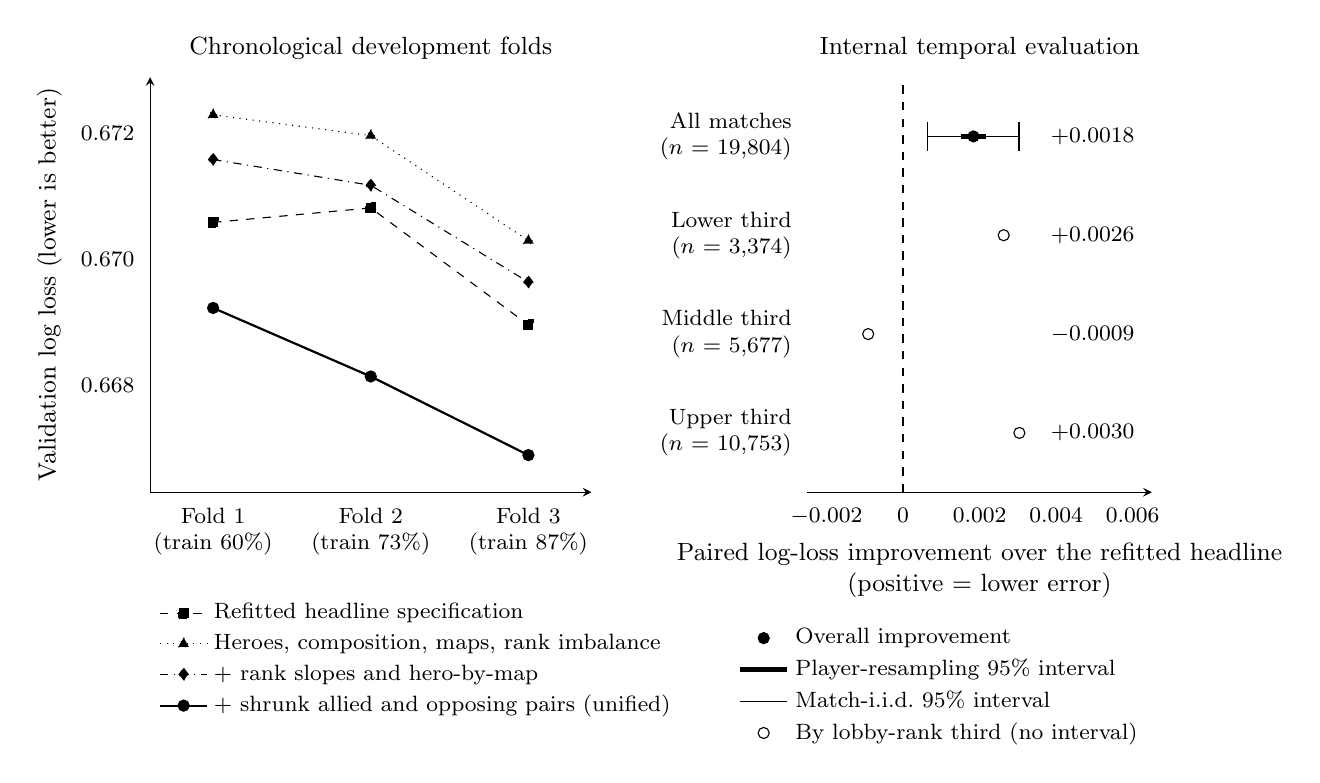
\begin{tikzpicture}
\begin{axis}[
  name=folds, scale only axis, width=159.5pt, height=150.0pt, axis lines=left, tick style={draw=none}, clip=false,
  symbolic x coords={F1,F2,F3}, xtick={F1,F2,F3}, enlarge x limits=0.2,
  xticklabels={{Fold 1\\(train 60\%)},{Fold 2\\(train 73\%)},{Fold 3\\(train 87\%)}}, xticklabel style={align=center, font=\footnotesize},
  ylabel={Validation log loss (lower is better)}, ylabel style={font=\small},
  yticklabel style={font=\footnotesize, /pgf/number format/fixed, /pgf/number format/fixed zerofill, /pgf/number format/precision=3}, scaled y ticks=false,
  ymin=0.6663, ymax=0.6729,
  title={\small Chronological development folds}, title style={yshift=-3pt},
  legend style={at={(0,-0.24)}, anchor=north west, draw=none, fill=none, font=\footnotesize, cells={anchor=west}}, legend cell align=left,
]
\addplot[dashed, mark=square*, mark size=1.8pt] coordinates {(F1,0.67059) (F2,0.67082) (F3,0.66896)};
\addlegendentry{Refitted headline specification}
\addplot[dotted, mark=triangle*, mark size=2.2pt] coordinates {(F1,0.67230) (F2,0.67197) (F3,0.67030)};
\addlegendentry{Heroes, composition, maps, rank imbalance}
\addplot[dashdotted, mark=diamond*, mark size=2.2pt] coordinates {(F1,0.67159) (F2,0.67118) (F3,0.66964)};
\addlegendentry{+ rank slopes and hero-by-map}
\addplot[thick, mark=*, mark size=1.8pt] coordinates {(F1,0.66923) (F2,0.66814) (F3,0.66689)};
\addlegendentry{+ shrunk allied and opposing pairs (unified)}
\end{axis}
\begin{axis}[
  name=ev, at={(folds.south east)}, anchor=south west, xshift=78.0pt, scale only axis, width=124.5pt, height=150.0pt,
  axis lines=left, tick style={draw=none}, y axis line style={draw=none}, clip=false,
  xmin=-0.0025, xmax=0.0065, ymin=0.4, ymax=4.6, ytick={4,3,2,1}, yticklabels={{All matches\\($n$ = 19,804)},{Lower third\\($n$ = 3,374)},{Middle third\\($n$ = 5,677)},{Upper third\\($n$ = 10,753)}}, yticklabel style={align=right, font=\footnotesize},
  xtick={-0.002,0,0.002,0.004,0.006}, xticklabel style={font=\footnotesize, /pgf/number format/fixed, /pgf/number format/precision=3}, scaled x ticks=false,
  xlabel={Paired log-loss improvement over the refitted headline\\(positive = lower error)}, xlabel style={font=\small, align=center},
  title={\small Internal temporal evaluation}, title style={yshift=-3pt},
  legend style={at={(1,-0.3)}, anchor=north east, draw=none, fill=none, font=\footnotesize, cells={anchor=west}}, legend cell align=left,
]
\draw[dashed, thin] (axis cs:0,0.4) -- (axis cs:0,4.6);
\draw[thin] (axis cs:0.00064,4) -- (axis cs:0.00303,4);
\draw[thin] (axis cs:0.00064,3.85) -- (axis cs:0.00064,4.15); \draw[thin] (axis cs:0.00303,3.85) -- (axis cs:0.00303,4.15);
\draw[line width=1.8pt] (axis cs:0.00151,4) -- (axis cs:0.00217,4);
\addplot[only marks, mark=*, mark size=2pt] coordinates {(0.00184,4)};
\addlegendentry{Overall improvement}
\addlegendimage{line width=1.8pt}
\addlegendentry{Player-resampling 95\% interval}
\addlegendimage{thin}
\addlegendentry{Match-i.i.d.\ 95\% interval}
\addplot[only marks, mark=o, mark size=2pt] coordinates {(0.00263,3) (-0.00091,2) (0.00304,1)};
\addlegendentry{By lobby-rank third (no interval)}
\node[anchor=east, font=\footnotesize] at (axis cs:0.0063,4) {+0.0018};
\node[anchor=east, font=\footnotesize] at (axis cs:0.0063,3) {+0.0026};
\node[anchor=east, font=\footnotesize] at (axis cs:0.0063,2) {$-$0.0009};
\node[anchor=east, font=\footnotesize] at (axis cs:0.0063,1) {+0.0030};
\end{axis}
\end{tikzpicture}


\begin{minipage}{0.95\linewidth}\footnotesize\vspace{2pt}
\emph{Notes.} Left: validation log loss on three chronological development folds for the refitted headline
specification and for the unified model with successively larger blocks. Right: paired per-match log-loss
improvement of the unified model over the refitted headline on the <<N_CONF>> matches of the internal
temporal evaluation, overall with two 95\% intervals (one treating matches as independent, one resampling
players so that matches sharing players move together) and by lobby-rank third without intervals. Positive
values mean lower prediction error.
\end{minipage}
\end{figure}

The right panel is an internal temporal evaluation rather than a clean future test. The <<N_CONF>> matches
are those played in the final four days of the snapshot, after <<CONF_CUT>> UTC. Their outcomes were kept
out of every design build, fold, tuning run, and table above, and were first read for the comparison in
Figure~\ref{fig:pred} (Figure~\ref{fig:fit} describes the same slice), but the same days overlap
the final week already examined in the earlier report on the headline specification, so the comparison
inherits that prior use. On those matches the unified model's paired log-loss improvement over the
refitted headline is <<CONF_D>>, with a player-resampling interval of <<CONF_LO>> to <<CONF_HI>>. By lobby
third the improvement is <<CONF_D0>> in the lower third, <<CONF_D1>> in the middle, and <<CONF_D2>> in the
upper, the middle third being the one place where the headline specification did slightly better.

Calibration is summarised in Table~\ref{tab:cal}. A slope of one means predicted probabilities are neither
too confident nor too timid; the unified model's slopes sit near one on the development folds and at
<<CONF_SLOPE>> on the evaluation, rising to <<CONF_SLOPE2>> in the upper third. Saved calibration bins are
not available for the unified fit, so no calibration curve is drawn.

\begin{table}[H]\centering\small
\caption{Calibration slopes of the unified model (ideal value one)}\label{tab:cal}
\begin{tabular}{l r r r r}
\toprule
Sample & Overall & Lower third & Middle third & Upper third \\
\midrule
<<CAL_ROWS>>
\bottomrule
\end{tabular}
\end{table}

Figure~\ref{fig:fit} looks at the same evaluation slice from the side of the heroes, as the earlier report did
for its holdout week. Each of the <<N_CONF>> matches contributes two team-sides. Grouping team-sides by each
hero they started and comparing the model's mean predicted win probability with the share that actually won
gives one point per hero; grouping by composition shape gives one per shape. Across heroes the correlation
is <<FIT_HERO_CORR>> and the mean absolute gap <<FIT_HERO_GAP>> percentage points, against <<FIT_HERO_CORR_BASE>>
and <<FIT_HERO_GAP_BASE>> for the refitted headline specification, which shares the hero terms: at this level
of aggregation the two models are not distinguishable, and the improvement in Figure~\ref{fig:pred} is not
a matter of ranking heroes better. Across composition shapes the correlation is <<FIT_SHAPE_CORR>>.

\begin{figure}[!tb]\centering
\caption{Does the model predict which heroes' teams win? By starting hero and by composition}
\label{fig:fit}
\vspace{2pt}
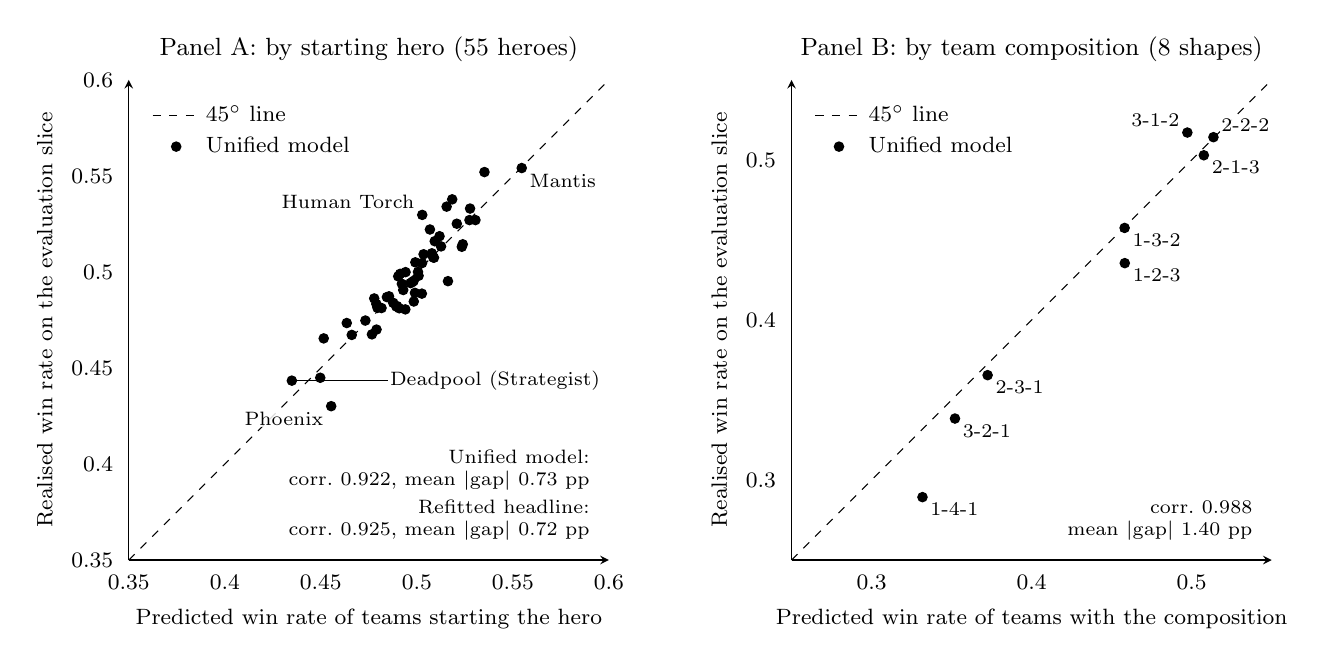
\begin{tikzpicture}
\begin{axis}[
  name=A, scale only axis, width=173.5pt, height=173.5pt, axis lines=left, tick style={draw=none}, clip=false,
  xmin=0.35, xmax=0.60, ymin=0.35, ymax=0.60,
  title={\small Panel A: by starting hero (55 heroes)}, title style={yshift=-3pt},
  xlabel={Predicted win rate of teams starting the hero}, ylabel={Realised win rate on the evaluation slice},
  label style={font=\footnotesize}, tick label style={font=\footnotesize, /pgf/number format/fixed, /pgf/number format/precision=2},
  legend style={at={(0.03,0.97)}, anchor=north west, font=\footnotesize, draw=none, fill=none, cells={anchor=west}},
]
\addplot[dashed, thin, domain=0.35:0.60, samples=2] {x};
\addlegendentry{$45^\circ$ line}
\addplot[only marks, mark=*, mark size=1.7pt] table[x=p, y=a] {
p a
0.4983 0.4953
0.4893 0.4820
0.5208 0.5251
0.5184 0.5378
0.5028 0.5297
0.4940 0.4805
0.5546 0.5541
0.4790 0.4700
0.4897 0.4822
0.5305 0.5270
0.4984 0.4846
0.5009 0.4980
0.4789 0.4833
0.4967 0.4942
0.5274 0.5270
0.5277 0.5330
0.5026 0.4887
0.4766 0.4675
0.4635 0.4734
0.4922 0.4938
0.5068 0.5221
0.4844 0.4869
0.4941 0.4999
0.5078 0.5097
0.4661 0.4672
0.5085 0.5076
0.5162 0.4952
0.4990 0.4891
0.5239 0.5144
0.5027 0.5046
0.4913 0.4990
0.4778 0.4862
0.5234 0.5131
0.4795 0.4813
0.4855 0.4873
0.5006 0.5000
0.4929 0.4906
0.5352 0.5520
0.5089 0.5074
0.4816 0.4812
0.4554 0.4301
0.5118 0.5186
0.5093 0.5160
0.5035 0.5092
0.4976 0.4947
0.4732 0.4747
0.5155 0.5340
0.4908 0.4811
0.4497 0.4449
0.4903 0.4977
0.4992 0.5050
0.5126 0.5133
0.4515 0.4654
0.4877 0.4839
0.4349 0.4434
};
\addlegendentry{Unified model}
\draw[very thin] (axis cs:0.4349,0.4434) -- (axis cs:0.4849,0.4434);
\node[font=\scriptsize, anchor=west, inner sep=0.6pt, fill=white, fill opacity=0.85, text opacity=1] at (axis cs:0.4849,0.4434) {Deadpool (Strategist)};
\node[font=\scriptsize, anchor=north east, inner sep=0.6pt, fill=white, fill opacity=0.85, text opacity=1] at (axis cs:0.4524,0.4281) {Phoenix};
\node[font=\scriptsize, anchor=south east, inner sep=0.6pt, fill=white, fill opacity=0.85, text opacity=1] at (axis cs:0.4998,0.5317) {Human Torch};
\node[font=\scriptsize, anchor=north west, inner sep=0.6pt, fill=white, fill opacity=0.85, text opacity=1] at (axis cs:0.5576,0.5521) {Mantis};
\node[anchor=south east, align=right, font=\scriptsize] at (rel axis cs:0.98,0.02)
  {Unified model:\\ corr.\ 0.922, mean $|$gap$|$ 0.73 pp\\[2pt] Refitted headline:\\ corr.\ 0.925, mean $|$gap$|$ 0.72 pp};
\end{axis}
\begin{axis}[
  name=B, at={(A.south east)}, anchor=south west, xshift=66.0pt, scale only axis, width=173.5pt, height=173.5pt,
  axis lines=left, tick style={draw=none}, clip=false,
  xmin=0.25, xmax=0.55, ymin=0.25, ymax=0.55,
  title={\small Panel B: by team composition (8 shapes)}, title style={yshift=-3pt},
  xlabel={Predicted win rate of teams with the composition}, ylabel={Realised win rate on the evaluation slice},
  label style={font=\footnotesize}, tick label style={font=\footnotesize, /pgf/number format/fixed, /pgf/number format/precision=2},
  legend style={at={(0.03,0.97)}, anchor=north west, font=\footnotesize, draw=none, fill=none, cells={anchor=west}},
]
\addplot[dashed, thin, domain=0.25:0.55, samples=2] {x};
\addlegendentry{$45^\circ$ line}
\addplot[only marks, mark=*, mark size=1.7pt] table[x=p, y=a] {
p a
0.4582 0.4355
0.4581 0.4575
0.3318 0.2893
0.5076 0.5029
0.5136 0.5142
0.3725 0.3655
0.4973 0.5171
0.3521 0.3384
};
\addlegendentry{Unified model}
\node[font=\scriptsize, anchor=north west, inner sep=0.6pt, fill=white, fill opacity=0.85, text opacity=1] at (axis cs:0.3354,0.2869) {1-4-1};
\node[font=\scriptsize, anchor=north west, inner sep=0.6pt, fill=white, fill opacity=0.85, text opacity=1] at (axis cs:0.3557,0.3360) {3-2-1};
\node[font=\scriptsize, anchor=north west, inner sep=0.6pt, fill=white, fill opacity=0.85, text opacity=1] at (axis cs:0.3761,0.3631) {2-3-1};
\node[font=\scriptsize, anchor=north west, inner sep=0.6pt, fill=white, fill opacity=0.85, text opacity=1] at (axis cs:0.4617,0.4551) {1-3-2};
\node[font=\scriptsize, anchor=north west, inner sep=0.6pt, fill=white, fill opacity=0.85, text opacity=1] at (axis cs:0.4618,0.4331) {1-2-3};
\node[font=\scriptsize, anchor=south east, inner sep=0.6pt, fill=white, fill opacity=0.85, text opacity=1] at (axis cs:0.4937,0.5195) {3-1-2};
\node[font=\scriptsize, anchor=north west, inner sep=0.6pt, fill=white, fill opacity=0.85, text opacity=1] at (axis cs:0.5112,0.5005) {2-1-3};
\node[font=\scriptsize, anchor=south west, inner sep=0.6pt, fill=white, fill opacity=0.85, text opacity=1] at (axis cs:0.5172,0.5166) {2-2-2};
\node[anchor=south east, align=right, font=\scriptsize] at (rel axis cs:0.98,0.02)
  {corr.\ 0.988\\ mean $|$gap$|$ 1.40 pp};
\end{axis}
\end{tikzpicture}


\begin{minipage}{0.95\linewidth}\footnotesize\vspace{2pt}
\emph{Notes.} The <<N_CONF>> matches of the internal temporal evaluation, each contributing two team-sides;
predictions are from the selected fit on development rows. Panel A groups team-sides by each hero they started:
the horizontal axis is the unified model's mean predicted win probability for those team-sides, the vertical
axis the share that actually won. Labels mark the two heroes farthest from the line and the two extremes; the
smallest hero group has <<FIT_MIN_HERO_SIDES>> team-sides, so a realised share can miss its prediction by a
point or two through sampling alone. Panel B groups team-sides by composition shape (Tanks--Damage--Supports)
with at least <<FIT_MIN_SIDES>> team-sides. The refitted headline specification's statistics are shown for
comparison; its points are not drawn because they sit on top of the unified model's.
\end{minipage}
\end{figure}

\section*{What remains uncertain?}

Two kinds of uncertainty are involved, and only one has been computed. The interval on the evaluation's
average improvement comes from resampling players so that matches sharing players move together. The
stability of individual hero and pair estimates under the same resampling is a separate exercise; at the
time of this build it had completed <<BOOT_REPS>> replications and is not reported, so no figure in this
report carries confidence bands or significance marks, and differences of a few tenths of a point between
heroes, or a few hundredths in pair contrasts, should be treated as unresolved.

The estimates describe the sampled competitive environment, not the whole ranked population. Lobby means
run from <<LOB_P5>> at the 5th percentile to <<LOB_P95>> at the 95th, no sampled player scores above
5{,}750, and the crawl reaches players only through public profiles, so the top of the ladder is absent
and nothing here should be extrapolated to it. Hero choice is also not random: rank score adjusts for broad
differences in player strength, not for a player's skill on the specific hero, and coordinated groups may
choose particular pairs. The pair contrasts therefore combine kit complementarity with who plays the pair
and when.

The sample was checked against the official patch record: the Season 9.5 balance state ran from 7 August to
the Season 10 patch on 11 September, and the five updates in between were cosmetic. A weekly win-rate
check flags only The Hood, released on 7 August, whose win rate drifted over the season; the audit
establishes that no identified balance change coincided with the drift, not what caused it. Matches in
which two teammates share the same first-appearance hero, <<N_ILLEGAL>> in all, were excluded because such
a start cannot be simultaneous and the record is unverifiable. Finally, the evaluation above overlaps
data used earlier, as disclosed; a clean test needs matches played after the model was fixed, which the
Season 10 patch now makes a different balance regime. <<PUB_NOTE>>

\FloatBarrier
\appendix
\FloatBarrier
\section*{Appendix A. Data, regime, and protocol}

\textbf{Snapshot.} <<N_SNAP>> competitive PC ranked matches played between <<PLAY_MIN>> and <<PLAY_MAX>>
UTC, frozen on <<FROZEN>> with a manifest of file hashes. Filters: twelve players, six per side, no draws,
pre-match scores present, every player with positive play time, at least 240 seconds. The starting record
is taken from the first-appearance entry of each player's hero list; <<N_ILLEGAL>> matches with a
duplicated first-appearance hero within a side are excluded, leaving <<N_DESIGN>>.

\textbf{Regime.} Official patch pages place the snapshot inside one balance regime, from the Season 9.5
patch (7 August 09:00 UTC, which also introduced The Hood) to the Season 10 patch (11 September 09:00
UTC). Updates on 13, 20, and 27 August and 3 September were cosmetic or bug fixes.

\textbf{Development and evaluation split.} Development rows are the <<N_DEV>> matches played up to
<<CONF_CUT>> UTC; the evaluation slice is the <<N_CONF>> played afterward. Collection was paused before
the rebuild, so the slice is internal to the snapshot. The candidate's specification, penalties, and
coefficients were hashed into a lock file (<<LOCK_HASH>>, <<LOCK_TIME>> UTC) before the slice's outcomes
were read, and the evaluator refuses to run twice. The predeclared comparison was a paired log-loss
improvement with a player-resampling interval excluding zero, calibration slope between 0.85 and 1.15
overall and by third, and no third worse than $-0.001$; all held. The baseline for the comparison is the
headline specification refitted on the development rows, because its published fit had used the whole
snapshot. As stated in the main text, the slice overlaps data examined in the earlier report.

\textbf{Rank coverage.} Table~\ref{tab:cov} gives the distribution of lobby means and individual scores.
<<N_ABOVE_5000>> matches have a lobby mean above 5{,}000 and <<N_PL_5500>> distinct players score above
5{,}500; no player scores above 5{,}750.

\begin{table}[H]\centering\small
\caption{Rank coverage of the development snapshot (pre-match scores)}\label{tab:cov}
\begin{tabular}{l r r r r r r r}
\toprule
& p5 & p25 & p50 & p75 & p95 & p99 & max \\
\midrule
<<COV_ROWS>>
\bottomrule
\end{tabular}
\end{table}

\section*{Appendix B. Model, identification, and penalty search}

Let $A_{mh}$ and $B_{mh}$ indicate whether hero $h$ starts on side~0 or side~1 of match $m$, $r_m$ the
standardized lobby rank, $\Delta R_m$ the standardized difference in team mean pre-match score, $v_m$ the
map, and $c(\cdot)$ the composition. With $x_{mh}=A_{mh}-B_{mh}$, $z_{mhk}=A_{mh}A_{mk}-B_{mh}B_{mk}$, and
$w_{mhk}=A_{mh}B_{mk}-A_{mk}B_{mh}$ for $h<k$,
\begin{align*}
\operatorname{logit}p_m ={}& \alpha_{v_m}+(\theta_0+\theta_1 r_m)\Delta R_m
 +(\gamma_0+\gamma_1 r_m)^\top[c(A_m)-c(B_m)]
 +\sum_h(\beta_h+d_h r_m+u_{h,v_m})\,x_{mh}\\
&+\sum_{h<k}(S_{hk}+T_{hk}r_m)\,z_{mhk}+\sum_{h<k}(C_{hk}+D_{hk}r_m)\,w_{mhk}.
\end{align*}
The allied block is symmetric and the opposing block antisymmetric, so swapping the two camps negates
every feature except the map intercept; the implementation checks this numerically. Every observed
composition shape, allied pair, opposing pair, and hero-by-map cell has a coefficient. The blocks are
aliased in known ways: summing a hero's allied features over five teammates gives five times its own
contrast, summing its opposing features over six opponents gives six times it, summing allied features
within a role pair gives a function of the composition contrast, and summing hero-by-map deviations over
maps gives the hero contrast again. Each candidate centering direction was tested against the data and
imposed only when its image lies exactly in the span of the lower-order blocks; <<N_CONSTRAINTS>> of
<<N_CANDIDATES>> candidates did, the largest residual being <<MAX_RESID>>, leaving <<N_FREE>> free
coefficients. Five ridge groups shrink the coefficients on their native scale: hero and composition
averages ($\lambda_1$), allied averages ($\lambda_2$), opposing averages ($\lambda_3$), hero and
composition rank slopes with hero-by-map deviations ($\lambda_4$), and pair rank slopes ($\lambda_5$);
map intercepts and the rank-imbalance terms are unpenalized. The rank basis and $\Delta R$ are scaled
with training rows only.

Penalties were tuned on the three chronological folds by a bounded coordinate search on $\log_{10}\lambda$
with warm starts, <<N_EVAL>> evaluations in all, the coarse passes on a half subsample of each fold's
training rows and the fine pass on full rows. The selected penalties are $\lambda=(<<LAMS>>)$. The
surface near the optimum is flat: the eight best full-row evaluations in Table~\ref{tab:tune} lie within
<<TUNE_SPREAD>> of each other. The selected fit converged to a coefficient change below $10^{-6}$ in
<<FINAL_ITERS>> Newton steps. Table~\ref{tab:ladder} gives the reduced-model ladder behind
Figure~\ref{fig:pred}.

\begin{table}[H]\centering\footnotesize
\caption{Best full-row evaluations of the penalty search}\label{tab:tune}
\begin{tabular}{l r r r}
\toprule
$\lambda_1,\lambda_2,\lambda_3,\lambda_4,\lambda_5$ & Mean validation log loss & Mean calibration slope & Converged \\
\midrule
<<TUNING_ROWS>>
\bottomrule
\end{tabular}
\end{table}

\begin{table}[H]\centering\footnotesize
\caption{Development ladder: genuine reduced fits at the selected penalties}\label{tab:ladder}
\begin{tabular}{l r r r r r r}
\toprule
Model & Free parameters & Fold 1 & Fold 2 & Fold 3 & Mean & Cal.\ slope \\
\midrule
<<LADDER_ROWS>>
\bottomrule
\end{tabular}
\end{table}

\textbf{Software metadata.} Design and fitter in the repository's \texttt{lineup} package at revision
<<CODE_REV>>; penalty search run on an 8-CPU Colab runtime from the cached design; report build
\texttt{<<BUILD>>}, the hash of this document's text with the hash itself left blank.

\section*{Appendix C. Full tables and figures}

\begin{landscape}
\begin{center}
{\scriptsize\setlength{\tabcolsep}{2.6pt}\renewcommand{\arraystretch}{1.06}
\captionof{table}{Hero coefficients and replacement values, all 55 heroes}\label{tab:hero}
\begin{tabular}{l r r r r r r r @{\hspace{1.6em}} l r r r r r r r}
\toprule
<<HERO_HDR>>
\midrule
<<HERO_BODY>>
\bottomrule
\end{tabular}
}
\end{center}
\vspace{-4pt}
\noindent\begin{minipage}{\linewidth}\footnotesize
\emph{Notes.} All 55 heroes are listed, sorted within role by the common-reference value. $\beta_h$ is the
within-role log-odds contrast at the median lobby score of <<LOB_P50>>, and \emph{slope} its change per
standard deviation of lobby rank (<<R_SD>> points). \emph{Common ref.} and \emph{Obs.\ incumbent} are the two
replacement benchmarks of the main text, in percentage points of win probability over <<POOL_N>>
development matches; \emph{Lower third} and \emph{Upper third} average the observed-incumbent value within
the lower and upper thirds of the sample by lobby rank (cut at <<THIRD_LO>> and <<THIRD_HI>>), as in
Figure~\ref{fig:rank-all}. \emph{Slots \%} is the share of same-role slots in which the hero was a legal
replacement; every hero was scored on at least <<MIN_CONTEXTS>> eligible slots. No uncertainty has been
computed for these values.
\end{minipage}
\end{landscape}

\begin{figure}[H]\centering
\caption{Replacement values by lobby rank: lower third against upper third, all 55 heroes}\label{fig:rank-all}
\vspace{2pt}
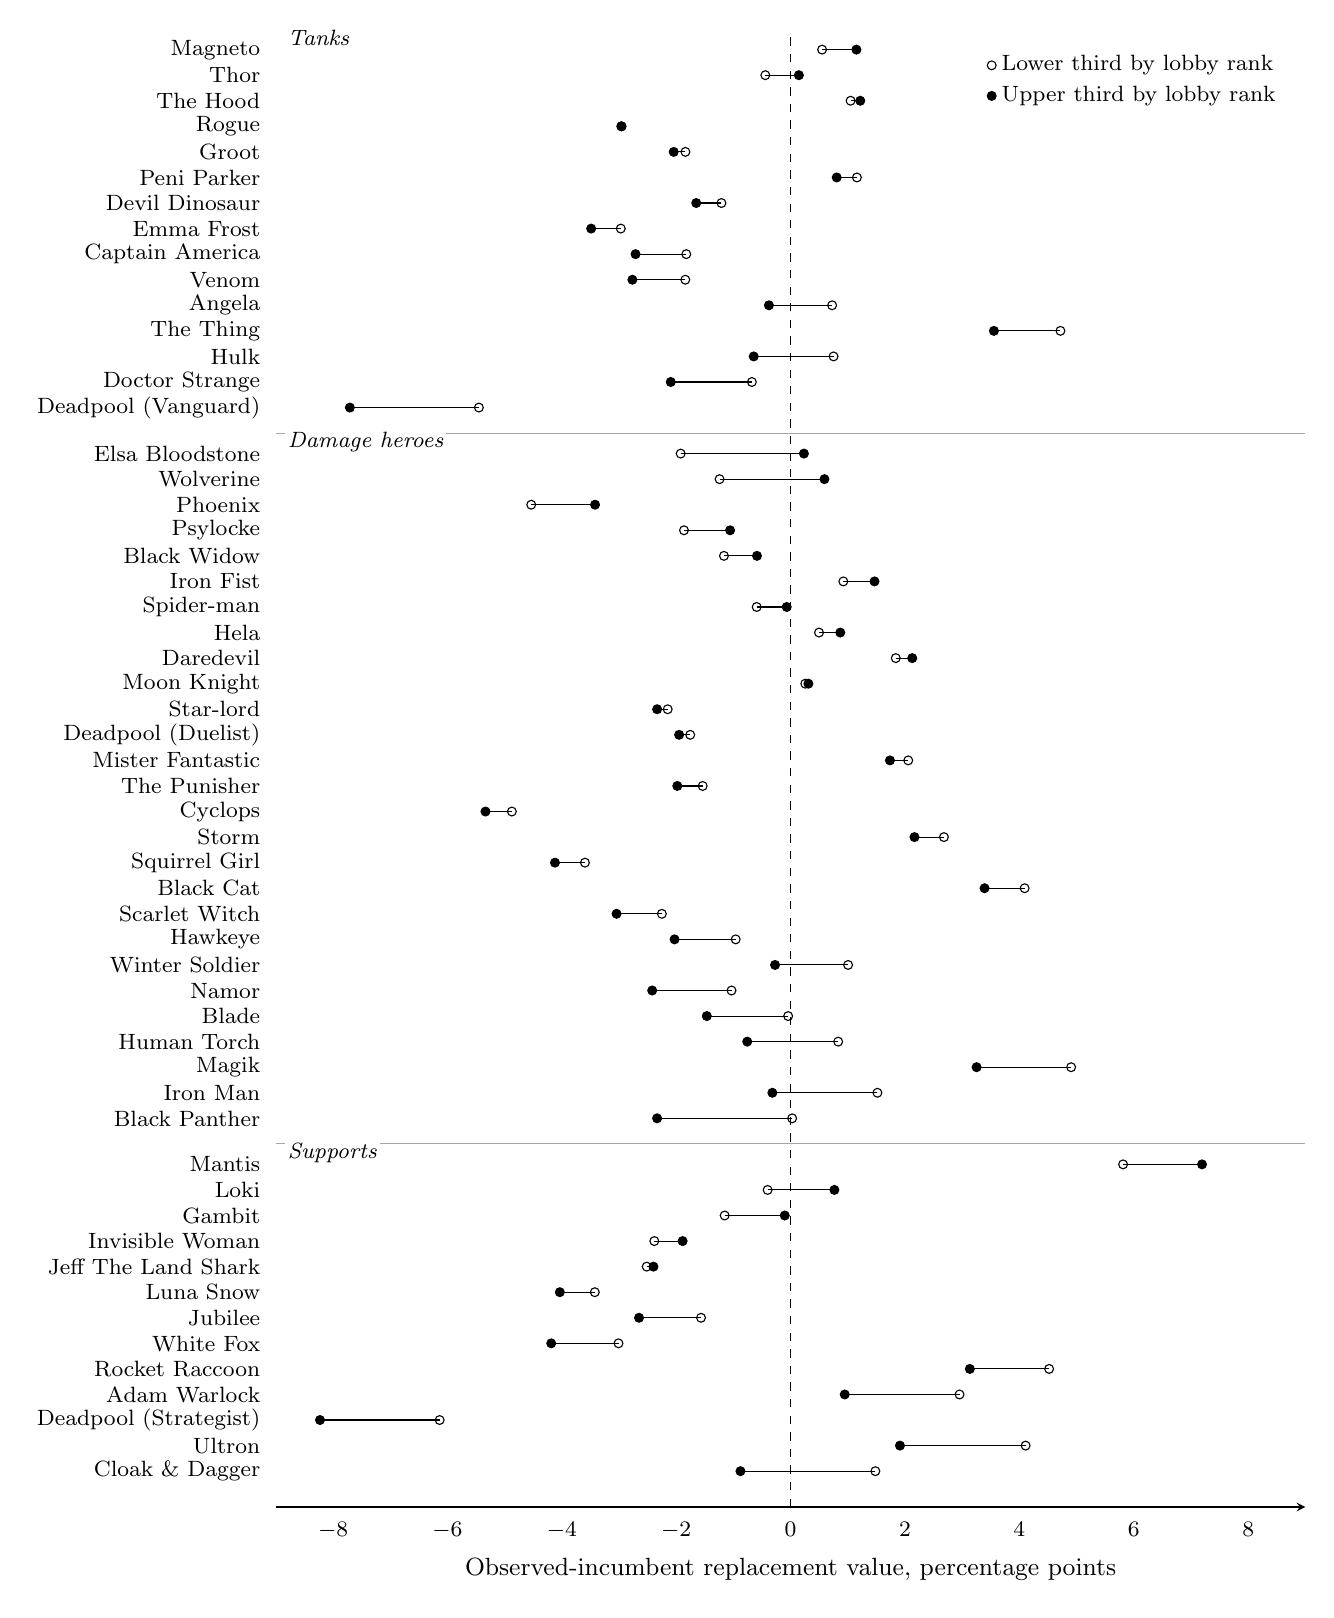
\begin{tikzpicture}
\begin{axis}[
  width=372.0pt, height=534.0pt, scale only axis, axis lines=left, tick style={draw=none}, y axis line style={draw=none}, clip=false,
  label style={font=\small}, tick label style={font=\footnotesize}, yticklabel style={font=\footnotesize},
  legend style={draw=none, fill=none, font=\footnotesize, cells={anchor=west}}, legend cell align=left,
  xmin=-9, xmax=9, ymin=0, ymax=57.80, xtick={-8,-6,...,8},
  xlabel={Observed-incumbent replacement value, percentage points},
  ytick={57.00,56.00,55.00,54.00,53.00,52.00,51.00,50.00,49.00,48.00,47.00,46.00,45.00,44.00,43.00,41.20,40.20,39.20,38.20,37.20,36.20,35.20,34.20,33.20,32.20,31.20,30.20,29.20,28.20,27.20,26.20,25.20,24.20,23.20,22.20,21.20,20.20,19.20,18.20,17.20,16.20,15.20,13.40,12.40,11.40,10.40,9.40,8.40,7.40,6.40,5.40,4.40,3.40,2.40,1.40}, yticklabels={{Magneto},{Thor},{The Hood},{Rogue},{Groot},{Peni Parker},{Devil Dinosaur},{Emma Frost},{Captain America},{Venom},{Angela},{The Thing},{Hulk},{Doctor Strange},{Deadpool (Vanguard)},{Elsa Bloodstone},{Wolverine},{Phoenix},{Psylocke},{Black Widow},{Iron Fist},{Spider-man},{Hela},{Daredevil},{Moon Knight},{Star-lord},{Deadpool (Duelist)},{Mister Fantastic},{The Punisher},{Cyclops},{Storm},{Squirrel Girl},{Black Cat},{Scarlet Witch},{Hawkeye},{Winter Soldier},{Namor},{Blade},{Human Torch},{Magik},{Iron Man},{Black Panther},{Mantis},{Loki},{Gambit},{Invisible Woman},{Jeff The Land Shark},{Luna Snow},{Jubilee},{White Fox},{Rocket Raccoon},{Adam Warlock},{Deadpool (Strategist)},{Ultron},{Cloak \& Dagger}},
  legend style={at={(0.985,0.99)}, anchor=north east},
]
\draw[dashed, thin] (axis cs:0,0) -- (axis cs:0,57.80);
\draw[black!35, thin] (axis cs:-9,42.00) -- (axis cs:9,42.00);
\draw[black!35, thin] (axis cs:-9,14.20) -- (axis cs:9,14.20);
\draw[thin] (axis cs:0.551,57.00) -- (axis cs:1.151,57.00);
\draw[thin] (axis cs:-0.442,56.00) -- (axis cs:0.145,56.00);
\draw[thin] (axis cs:1.049,55.00) -- (axis cs:1.218,55.00);
\draw[thin] (axis cs:-2.955,54.00) -- (axis cs:-2.960,54.00);
\draw[thin] (axis cs:-1.839,53.00) -- (axis cs:-2.044,53.00);
\draw[thin] (axis cs:1.159,52.00) -- (axis cs:0.806,52.00);
\draw[thin] (axis cs:-1.209,51.00) -- (axis cs:-1.650,51.00);
\draw[thin] (axis cs:-2.969,50.00) -- (axis cs:-3.487,50.00);
\draw[thin] (axis cs:-1.824,49.00) -- (axis cs:-2.711,49.00);
\draw[thin] (axis cs:-1.841,48.00) -- (axis cs:-2.766,48.00);
\draw[thin] (axis cs:0.726,47.00) -- (axis cs:-0.379,47.00);
\draw[thin] (axis cs:4.718,46.00) -- (axis cs:3.555,46.00);
\draw[thin] (axis cs:0.751,45.00) -- (axis cs:-0.645,45.00);
\draw[thin] (axis cs:-0.677,44.00) -- (axis cs:-2.095,44.00);
\draw[thin] (axis cs:-5.450,43.00) -- (axis cs:-7.706,43.00);
\draw[thin] (axis cs:-1.922,41.20) -- (axis cs:0.233,41.20);
\draw[thin] (axis cs:-1.242,40.20) -- (axis cs:0.592,40.20);
\draw[thin] (axis cs:-4.535,39.20) -- (axis cs:-3.419,39.20);
\draw[thin] (axis cs:-1.864,38.20) -- (axis cs:-1.058,38.20);
\draw[thin] (axis cs:-1.165,37.20) -- (axis cs:-0.588,37.20);
\draw[thin] (axis cs:0.922,36.20) -- (axis cs:1.467,36.20);
\draw[thin] (axis cs:-0.593,35.20) -- (axis cs:-0.068,35.20);
\draw[thin] (axis cs:0.497,34.20) -- (axis cs:0.869,34.20);
\draw[thin] (axis cs:1.839,33.20) -- (axis cs:2.127,33.20);
\draw[thin] (axis cs:0.257,32.20) -- (axis cs:0.311,32.20);
\draw[thin] (axis cs:-2.149,31.20) -- (axis cs:-2.334,31.20);
\draw[thin] (axis cs:-1.755,30.20) -- (axis cs:-1.949,30.20);
\draw[thin] (axis cs:2.057,29.20) -- (axis cs:1.737,29.20);
\draw[thin] (axis cs:-1.537,28.20) -- (axis cs:-1.981,28.20);
\draw[thin] (axis cs:-4.874,27.20) -- (axis cs:-5.335,27.20);
\draw[thin] (axis cs:2.681,26.20) -- (axis cs:2.166,26.20);
\draw[thin] (axis cs:-3.596,25.20) -- (axis cs:-4.120,25.20);
\draw[thin] (axis cs:4.092,24.20) -- (axis cs:3.391,24.20);
\draw[thin] (axis cs:-2.251,23.20) -- (axis cs:-3.043,23.20);
\draw[thin] (axis cs:-0.960,22.20) -- (axis cs:-2.029,22.20);
\draw[thin] (axis cs:1.005,21.20) -- (axis cs:-0.272,21.20);
\draw[thin] (axis cs:-1.033,20.20) -- (axis cs:-2.420,20.20);
\draw[thin] (axis cs:-0.043,19.20) -- (axis cs:-1.465,19.20);
\draw[thin] (axis cs:0.832,18.20) -- (axis cs:-0.758,18.20);
\draw[thin] (axis cs:4.905,17.20) -- (axis cs:3.252,17.20);
\draw[thin] (axis cs:1.518,16.20) -- (axis cs:-0.319,16.20);
\draw[thin] (axis cs:0.027,15.20) -- (axis cs:-2.334,15.20);
\draw[thin] (axis cs:5.813,13.40) -- (axis cs:7.194,13.40);
\draw[thin] (axis cs:-0.402,12.40) -- (axis cs:0.766,12.40);
\draw[thin] (axis cs:-1.153,11.40) -- (axis cs:-0.102,11.40);
\draw[thin] (axis cs:-2.383,10.40) -- (axis cs:-1.888,10.40);
\draw[thin] (axis cs:-2.516,9.40) -- (axis cs:-2.398,9.40);
\draw[thin] (axis cs:-3.423,8.40) -- (axis cs:-4.035,8.40);
\draw[thin] (axis cs:-1.566,7.40) -- (axis cs:-2.650,7.40);
\draw[thin] (axis cs:-3.009,6.40) -- (axis cs:-4.185,6.40);
\draw[thin] (axis cs:4.520,5.40) -- (axis cs:3.134,5.40);
\draw[thin] (axis cs:2.954,4.40) -- (axis cs:0.946,4.40);
\draw[thin] (axis cs:-6.136,3.40) -- (axis cs:-8.228,3.40);
\draw[thin] (axis cs:4.109,2.40) -- (axis cs:1.912,2.40);
\draw[thin] (axis cs:1.482,1.40) -- (axis cs:-0.877,1.40);
\addplot[only marks, mark=o, mark size=1.6pt] coordinates {
(0.551,57.00)
(-0.442,56.00)
(1.049,55.00)
(-2.955,54.00)
(-1.839,53.00)
(1.159,52.00)
(-1.209,51.00)
(-2.969,50.00)
(-1.824,49.00)
(-1.841,48.00)
(0.726,47.00)
(4.718,46.00)
(0.751,45.00)
(-0.677,44.00)
(-5.450,43.00)
(-1.922,41.20)
(-1.242,40.20)
(-4.535,39.20)
(-1.864,38.20)
(-1.165,37.20)
(0.922,36.20)
(-0.593,35.20)
(0.497,34.20)
(1.839,33.20)
(0.257,32.20)
(-2.149,31.20)
(-1.755,30.20)
(2.057,29.20)
(-1.537,28.20)
(-4.874,27.20)
(2.681,26.20)
(-3.596,25.20)
(4.092,24.20)
(-2.251,23.20)
(-0.960,22.20)
(1.005,21.20)
(-1.033,20.20)
(-0.043,19.20)
(0.832,18.20)
(4.905,17.20)
(1.518,16.20)
(0.027,15.20)
(5.813,13.40)
(-0.402,12.40)
(-1.153,11.40)
(-2.383,10.40)
(-2.516,9.40)
(-3.423,8.40)
(-1.566,7.40)
(-3.009,6.40)
(4.520,5.40)
(2.954,4.40)
(-6.136,3.40)
(4.109,2.40)
(1.482,1.40)
};
\addlegendentry{Lower third by lobby rank}
\addplot[only marks, mark=*, mark size=1.6pt] coordinates {
(1.151,57.00)
(0.145,56.00)
(1.218,55.00)
(-2.960,54.00)
(-2.044,53.00)
(0.806,52.00)
(-1.650,51.00)
(-3.487,50.00)
(-2.711,49.00)
(-2.766,48.00)
(-0.379,47.00)
(3.555,46.00)
(-0.645,45.00)
(-2.095,44.00)
(-7.706,43.00)
(0.233,41.20)
(0.592,40.20)
(-3.419,39.20)
(-1.058,38.20)
(-0.588,37.20)
(1.467,36.20)
(-0.068,35.20)
(0.869,34.20)
(2.127,33.20)
(0.311,32.20)
(-2.334,31.20)
(-1.949,30.20)
(1.737,29.20)
(-1.981,28.20)
(-5.335,27.20)
(2.166,26.20)
(-4.120,25.20)
(3.391,24.20)
(-3.043,23.20)
(-2.029,22.20)
(-0.272,21.20)
(-2.420,20.20)
(-1.465,19.20)
(-0.758,18.20)
(3.252,17.20)
(-0.319,16.20)
(-2.334,15.20)
(7.194,13.40)
(0.766,12.40)
(-0.102,11.40)
(-1.888,10.40)
(-2.398,9.40)
(-4.035,8.40)
(-2.650,7.40)
(-4.185,6.40)
(3.134,5.40)
(0.946,4.40)
(-8.228,3.40)
(1.912,2.40)
(-0.877,1.40)
};
\addlegendentry{Upper third by lobby rank}
\node[anchor=west, font=\footnotesize\itshape, fill=white, inner sep=1pt] at (axis cs:-8.85,57.45) {Tanks};
\node[anchor=west, font=\footnotesize\itshape, fill=white, inner sep=1pt] at (axis cs:-8.85,41.65) {Damage heroes};
\node[anchor=west, font=\footnotesize\itshape, fill=white, inner sep=1pt] at (axis cs:-8.85,13.85) {Supports};
\end{axis}
\end{tikzpicture}


\begin{minipage}{0.95\linewidth}\footnotesize\vspace{2pt}
\emph{Notes.} Observed-incumbent replacement values from the selected fit, averaged within the lower and
upper thirds of sampled lobbies by mean pre-match score (cut at <<THIRD_LO>> and <<THIRD_HI>>). Within each
role, heroes are sorted by the change from the lower to the upper third. Lines join two estimates from the
same fit and are not confidence intervals; no uncertainty has been computed for these values.
\end{minipage}
\end{figure}

\begin{landscape}
\begin{center}
{\scriptsize\setlength{\tabcolsep}{2.8pt}\renewcommand{\arraystretch}{1.0}
\captionof{table}{Team-up-eligible allied pairs with at least <<MIN_SUPPORT>> identifying matches, all <<N_TU>> pairs}\label{tab:tu}
\begin{tabular}{l r r @{\hspace{1em}} l r r @{\hspace{1em}} l r r}
\toprule
<<TU_HDR>>
\midrule
<<TU_BODY>>
\bottomrule
\end{tabular}
}
\end{center}
\vspace{-2pt}
\noindent\begin{minipage}{\linewidth}\footnotesize
\emph{Notes.} Pairs are listed in descending order of contrast, reading down each column in turn.
\emph{Contrast} is the four-lineup log-odds contrast at the median lobby rank and \emph{Matches} the number
of distinct development matches with a nonzero signed feature. Read as the synergy of a team-up-eligible
starting pair; activation of the team-up ability is not observed.
\end{minipage}
\end{landscape}

\begin{landscape}
\begin{center}
{\footnotesize\setlength{\tabcolsep}{3.5pt}\renewcommand{\arraystretch}{1.0}
\captionof{table}{Other allied pairs: 25 largest positive and 25 largest negative contrasts}\label{tab:nt}
\begin{tabular}{l r r r @{\hspace{2em}} l r r r}
\toprule
\multicolumn{4}{l}{\emph{Largest positive}} & \multicolumn{4}{l}{\emph{Largest negative}} \\
Pair & Contrast & Matches & Top third \% & Pair & Contrast & Matches & Top third \% \\
\midrule
<<NT_ROWS>>
\bottomrule
\end{tabular}
}
\end{center}
\vspace{-2pt}
\noindent\begin{minipage}{\linewidth}\footnotesize
\emph{Notes.} \emph{Contrast} and \emph{Matches} as in Table~\ref{tab:tu}; \emph{Top third \%} is the share
of the identifying matches in the upper lobby-rank third. Pairs with at least <<MIN_SUPPORT>> identifying
matches that are not designated team-ups.
\end{minipage}
\end{landscape}

\begin{landscape}
\begin{center}
{\footnotesize\setlength{\tabcolsep}{3.5pt}\renewcommand{\arraystretch}{1.0}
\captionof{table}{Opposing matchups: 50 largest contrasts, oriented as A against B}\label{tab:opp}
\begin{tabular}{l r r r @{\hspace{2em}} l r r r}
\toprule
Matchup & Contrast & Matches & Top third \% & Matchup & Contrast & Matches & Top third \% \\
\midrule
<<O_ROWS>>
\bottomrule
\end{tabular}
}
\end{center}
\vspace{-2pt}
\noindent\begin{minipage}{\linewidth}\footnotesize
\emph{Notes.} Columns as in Table~\ref{tab:nt}. ``A against B'' means that A's side wins more often when
the two start on opposite sides than the heroes' other matchups predict.
\end{minipage}
\end{landscape}

\section*{Appendix D. Earlier-specification results on attribution rules}

The numbers here come from the earlier report's headline specification (starting-hero attribution,
within-role constraint, map intercepts, designated team-ups only), not from the unified model, and are
kept for reference. Fitting that specification under the three attribution rules of Figure~\ref{fig:swap}
on the same <<N_OLD>> matches gave cross-hero standard deviations of the within-role estimates of
<<OLD_SD0>> percentage points under starting-hero attribution, <<OLD_SD2>> under most-played attribution,
and <<OLD_SD1>> under time weighting; Magik's estimate moved from <<OLD_MAGIK0>> to <<OLD_MAGIK2>> to
<<OLD_MAGIK1>>. The rules that use more information from after the opening produce larger estimates, which
is consistent with swaps responding to the match, and is the reason the starting record is used here.

\end{document}
